%%
%% Edit the following two statements with the title of your report and the names of your team members.

\def\mytitle{The Star Solution}

\def\myauthor{Komi Agbo, Dalton Burke, Nick Mako, James Vance}


%%=========================================
%%
%%  Do no edit the following block
%%
%%VVVVVVVVVVVVVVVVVVVVVVVVVVVVVVVVVVVVVV

\ifdefined\CLINICMAIN
(by \myauthor)

\else

\documentclass{article}
\usepackage{graphicx}
%%%%%%%%%%%%%%%%%%%%%%%%%%%%%%%%%%%%%%%%%%%%%%%%%%%%%%%%%%%%%%%%%%%%%%%%
% clinicPreamble.tex    input to preamble of clinic report
% created 12-20-00 by Harvey J. Greenberg
%%%%%%%%%%%%%%%%%%%%%%%%%%%%%%%%%%%%%%%%%%%%%%%%%%%%%%%%%%%%%%%%%%%%%%%

% Packages that might be used

\usepackage{algorithmic}       % enables algorithm environment
\usepackage{amsbsy}            % allows bold + italic
\usepackage{amsmath}           % formerly amstex
\usepackage{amssymb}           % ams symbols (\mathbb fonts)
\usepackage{bibunits}          % enables multiple bibliographies
\usepackage{bm}                % bold math fonts (\mathbm)
\usepackage[T1]{fontenc}       % ...to write \textbf{\textsc{..}}
\usepackage{fancyvrb,moreverb} % verbatim
\usepackage{float}             % enable float [H] option
\usepackage{graphicx}          % graphics (pst-all can be added to use PStricks)
\usepackage{mathrsfs}          % more math symbols (viz., \mathscr)
\usepackage{multirow}          % like multicolumn
\usepackage{theorem}           % enables more control over newtheorem
\usepackage{url}               % \url{...}

% theorem package enables the following
{\theorembodyfont{\rmfamily} \newtheorem{example}{Example}[section]}
{\theorembodyfont{\rmfamily} \newtheorem{remark}{Remark}[section]}
{\theorembodyfont{\rmfamily} \newtheorem{definition}{Definition}[section]}
%                  ^ make text in definition roman (not italic)
\renewcommand\url{\begingroup\urlstyle{rm}\Url}  % puts url in rm font

%%%%%%%%%%%%%%%%%%%%%%%%%%%%% End Packages %%%%%%%%%%%%%%%%%%%%%%%%%%%%%%%%%%%

%%%%%%%%%%%%%%%%%%%%%%%%%%%%%%%%%%%%%%%%%%%%%%%%%%%%%%%%%%%%%%%%%%%%%%%
% file: clinicmacros.tex  input to clinicF00.tex
% created 12-20-00 by Harvey J. Greenberg
% Last update: 1-3-01
%%%%%%%%%%%%%%%%% Begin new theorems and environments %%%%%%%%%%%%%%%%%
\newcommand{\figref}[1]{Figure~\ref{fig:#1}}
\newcommand{\tabref}[1]{Table~\ref{tab:#1}}
%\newcommand{\eqref}[1]{(\ref{eq:#1})}
\newcommand{\eqrefs}[2]{(\ref{eq:#1})--(\ref{eq:#2})}
\newcommand{\thmref}[1]{Theorem~\ref{thm:#1}}
\newcommand{\lemref}[1]{Lemma~\ref{lem:#1}}
\newcommand{\defref}[1]{Definition~\ref{def:#1}}
\newcommand{\corref}[1]{Corollary~\ref{cor:#1}}
\newcommand{\propref}[1]{Proposition~\ref{prop:#1}}
\newcommand{\asref}[1]{Assumption~\ref{ass:#1}}
\newcommand{\asrefs}[2]{Assumptions~\ref{ass:#1}--\ref{ass:#2}}
\newcommand{\algref}[1]{Algorithm~\ref{alg:#1}}
\newcommand{\probref}[1]{(\ref{prob:#1})}
\newcommand{\secref}[1]{Section~\ref{sec:#1}}
\newcommand{\chapref}[1]{Chapter~\ref{chap:#1}}
\newcommand{\appref}[1]{Appendix~\ref{app:#1}}
\newcommand{\mylabel}[1]{\label{#1}}



\newtheorem{theorem}{Theorem}[section]
\newtheorem{corollary}{Corollary}[theorem]
\newtheorem{lemma}{Lemma}[section]
\newtheorem{proposition}{Proposition}[section]
\newtheorem{conjecture}{Conjecture}[section]
% definition, example and remark environments are defined in 
% clinicPreamble to have Roman text (put term being defined into italics)

\newenvironment{Srule}{\refstepcounter{rule} % cannot use rule for env name
         \medskip\par\noindent\textbf{Rule \therule.} } {\medskip}

\newenvironment{enum0}{\vspace{-.19in}\par
                  \begin{enumerate}\setlength{\itemsep}{-.06in} }
                      {\end{enumerate}}

\newenvironment{exercise}{ \refstepcounter{exercise} 
    \renewcommand{\labelenumi}{\theexercise.\theenumi} 
                          \begin{description}
                            \item [Exercise \theexercise.] }
                         {\end{description} 
    \renewcommand{\labelenumi}{\theenumi} }

% The following needs the following defined:
%    \title, \teacher-name, \teacher-e-mail, \teacher-web, \date
%
\newcommand{\makeclinictitle}{\vspace*{.6in} \begin{center}%
                {\Large\textbf{FINAL REPORT OF THE \\
                               UCDHSC MATHEMATICS CLINIC\\ \bigskip
                               \title}} \\ \bigskip
	                       {\large Taught by \\ \teachername        
                            \\  University of Colorado at Denver
			    \\  and Health Sciences Center 
                            \\ Department of Mathematical Sciences
                            \\ P.O. Box 173364
                            \\ Denver, CO 80217-3364
                            \\ \teacheremail
                     \\ \bigskip \bigskip
                       {\large Sponsored by \\ \sponsorname}
                     \\ \bigskip \bigskip \renewcommand{\arraystretch}{1.1}
                         \begin{tabular}{|c|} \hline
                             \textbf{Participating students:} \\
                              \students \\ \hline
                         \end{tabular} \renewcommand{\arraystretch}{1}
                     \\ \bigskip \bigskip
                              \date} \end{center} \bigskip }
\newcommand{\qed}{\hspace*{\fill}\rule{1.5ex}{1.5ex} }
%%%%%%%%%%%% End newenvironments that might be disabled %%%%%%%%%%%%%%

\newtheorem{algorithm}{Algorithm}
\newenvironment{proof}{ \noindent\textbf{Proof:} }
%                       {\hspace*{\fill}\rule{1.5ex}{1.5ex}  }
                      {                          }
%%%%%%%%%%%% End all newtheorem and newenvironment specs %%%%%%%%%%%%%

%%%%%%%%%%%%%%%%%%%%%%%%%%% Begin defs %%%%%%%%%%%%%%%%%%%%%%%%%%%%%%%

% Simply abbreviations:
%\def\mc{\multicolumn}
%\def\ol{\overline}    % must be in math mode
%\def\ul{\underline}   % "
%\def\ob{\overbrace}   % "
%\def\ub{\underbrace}  % "
%\def\dag{\mbox{$^\dagger$}}
%\def\Larrow{\mbox{$\longleftarrow$}}
%\def\Rarrow{\mbox{$\longrightarrow$}}
%\def\Small{\scriptsize}
%\def\st{\,:}
\def\st{\mbox{subject to}}
% Calligraphic font:
\def\cA{\ensuremath{{\cal{A}}}}
\def\cB{\ensuremath{{\cal{B}}}}
\def\cC{\ensuremath{{\cal{C}}}}
\def\cD{\ensuremath{{\cal{D}}}}
\def\cE{\ensuremath{{\cal{E}}}}
\def\cF{\ensuremath{{\cal{F}}}}
\def\cG{\ensuremath{{\cal{G}}}}
\def\cH{\ensuremath{{\cal{H}}}}
\def\cI{\ensuremath{{\cal{I}}}}
\def\cJ{\ensuremath{{\cal{J}}}}
\def\cK{\ensuremath{{\cal{K}}}}
\def\cL{\ensuremath{{\cal{L}}}}
\def\cM{\ensuremath{{\cal{M}}}}
\def\cN{\ensuremath{{\cal{N}}}}
\def\cO{\ensuremath{{\cal{O}}}}
\def\cP{\ensuremath{{\cal{P}}}}
\def\cQ{\ensuremath{{\cal{Q}}}}
\def\cR{\ensuremath{{\cal{R}}}}
\def\cS{\ensuremath{{\cal{S}}}}
\def\cT{\ensuremath{{\cal{T}}}}
\def\cU{\ensuremath{{\cal{U}}}}
\def\cV{\ensuremath{{\cal{V}}}}
\def\cW{\ensuremath{{\cal{W}}}}
\def\cX{\ensuremath{{\cal{X}}}}
\def\cY{\ensuremath{{\cal{Y}}}}
\def\cZ{\ensuremath{{\cal{Z}}}}

% The following were in latex but are not in latex2e:
\def\Box{\mbox{\begin{picture}(0,0) \put( 2,0){\framebox(7,7)} 
               \end{picture} }}
\def\lhd{\mbox{\large$\triangleleft$}}
\def\rhd{\mbox{\large$\triangleright$}}
\def\unlhd{\mbox{\underline{\large$\triangleleft$}}}
\def\unrhd{\mbox{\underline{\large$\triangleright$}}}
\def\Join{\mbox{$\triangleright\triangleleft$}}
\def\mho{\mbox{\hspace*{-.04in} \rotatebox[origin=c] {180} {$\Omega$} }}

% Other special characters:
\def\cents{\mbox{{\large$c\!\!$}{\small /} }}
\def\half{{\mbox{\small{$\frac{1}{2}$}}}}
\def\third{{\mbox{\small{$\frac{1}{3}$}}}}
\def\fourth{{\mbox{\small{$\frac{1}{4}$}}}}
\def\quarter{{\mbox{\small{$\frac{1}{4}$}}}}
\def\fifth{{\mbox{\small{$\frac{1}{5}$}}}}
\def\sixth{{\mbox{\small{$\frac{1}{6}$}}}}
\def\thrhlf{{\mbox{\small{$\frac{3}{2}$}}}}
\def\twothrd{{\mbox{\small{$\frac{2}{3}$}}}}
\def\forthrd{{\mbox{\small{$\frac{4}{3}$}}}}
\def\fivthrd{{\mbox{\small{$\frac{5}{3}$}}}}
\def\thrfrth{{\mbox{\small{$\frac{3}{4}$}}}}
\def\twoffth{{\mbox{\small{$\frac{2}{5}$}}}}
\def\thrffth{{\mbox{\small{$\frac{3}{5}$}}}}
\def\forffth{{\mbox{\small{$\frac{4}{5}$}}}}

\def\chkbox{\mbox{$\Box\hspace{-.2em}^\surd\;$}}
\def\defeq{\mbox{$\stackrel{\rm def}{=}$}}
\def\hence{\mbox{\footnotesize{$_\bullet$$^\bullet$$_\bullet$ }}}
%\def\LR{{\rlap{\rm I}\hskip0.11em\hbox{\rm R}}}
%\def\LZ{{\mbox{\rm\bf Z}}}
\newcommand\LR{\ensuremath{\mathbb{R}}}
\newcommand\LQ{\ensuremath{\mathbb{Q}}}
\newcommand\LZ{\ensuremath{\mathbb{Z}}}
\def\subdot{\mbox{\tiny$\bullet$}}
\def\swiggle{\mbox{$\zeta$}}

% The following enforce consistent notation in math mode:
\def\dim{\mbox{{\rm dim}}}           % dimension
%\def\rank{\mbox{{\rm rank}}}         % rank
%\def\nul{\cN}                        % null space
%\def\col{\mbox{{\rm col}}}           % column space
%\def\row{\mbox{{\rm row}}}           % row space
%\def\diag{\mbox{{\rm diag}}}         % diagonal matrix
\def\goto{\rightarrow}               % goto (limit or map)
\def\imply{\mbox{$\,\Rightarrow\,$}} % imply
\def\iff{\mbox{$\Leftrightarrow$}}   % if, and only if
\def\compl{\mbox{$^{_\sim}\!$}}      % complement (also for www)
\def\evec{\mbox{\rm{e}}}             % e-vector
\def\min{\mbox{\rm{min}}}            % minimize
\def\max{\mbox{\rm{max}}}            % maximize
\def\opt{\mbox{\rm{opt}}}            % optimize
\def\inf{\mbox{\rm{inf}}}            % infimum
\def\sup{\mbox{\rm{sup}}}            % supremum
%\def\argmax{\mbox{\rm{argmax}}}      % argmax
%\def\argmin{\mbox{\rm{argmin}}}      % argmin
\def\det{\mbox{\rm{det}}}            % determinate
%\def\ri{\mbox{\rm{ri}}}              % relative interior
\def\affh{\mbox{\rm{affh}}}          % affine hull
\def\convh{\mbox{\rm{convh}}}        % convex hull
\def\Ext{\mbox{\rm{Ext}}}            % extreme points
\def\Binv{{\mbox{$B^{-1}$}}}         % basis inverse
\def\transp{\ensuremath{^{\mathsf{T}}}} % transpose
%%%%%%%%%%%%%%%%%%%%%%%%%%% End defs %%%%%%%%%%%%%%%%%%%%%%%%%%%%%%%

%%%%%%%%%%%%%%%%%%% Begin newcommand specs %%%%%%%%%%%%%%%%%%%%%%%%%

% Functions:
\newcommand{\cmd}[1]{\mbox{$\backslash${\sf{#1}}}}
\newcommand{\norm}[1]{{\left\|{#1}\right\|}}
\newcommand{\Bigfrac}[2]{\mbox{$\frac{\mbox{$#1$}}{\mbox{$#2$}}$}}
\newcommand{\card}[1]{\mbox{\large{\bf $|$}}\mbox{$\{#1\}$}\mbox{\large{\bf $|$} }}
\newcommand{\intval}[1]{\mbox{$\left\lfloor #1 \right\rfloor$}}
\newcommand{\intup}[1]{\mbox{$\left\lceil #1 \right\rceil$}}
\newcommand{\vx}[2]{\mbox{$\left(\begin{array}{c}
                                    \!\!#1\!\! \\ \!\!#2\!\! 
                                 \end{array}\right)$ }}
\newcommand{\bi}[1]{\textit{\textbf{#1}}}
\newcommand{\vect}[2]{\left(\!\begin{array}{rr} #1 \\ 
                                                #2 \end{array}\!\right)}
\newcommand{\mbf}[1]{\mbox{{\boldmath$#1$}}}
\newcommand{\brackets}[1]{\left\{ {#1} \right\}}
\newcommand{\set}[2]{\brackets{{#1} \left|\; {#2} \right.}}


% Graphics & fonts
\newcommand{\usc}[1]{\ul{\hspace*{#1 in}}}
\newcommand\hr[1]{\vspace{-.2in}\begin{center}
                        \begin{tabular}{c}\hspace*{#1in} \\ \hline
                        \end{tabular}\end{center} }
\newcommand{\smiley}{  $\;\;\;^{\begin{picture}(0,0)
     \put(-8,0){\circle{9}}
     \put(-9,1){\circle*{1}} \put(-6,1){\circle*{1}}
     \put(-11.5,-3.6){\tiny$\smile$}
                             \end{picture} }$} 
\newcommand{\sadface}{ $\;\;\;^{\begin{picture}(0,0)
     \put(-8,0){\circle{9}}
     \put(-9,1){\circle*{1}} \put(-6,1){\circle*{1}}
     \put(-11.5,-3.6){\tiny$\frown$}
                             \end{picture}}$}
% The following allows me to put a note in the margin.
\newcommand{\MarginNote}[1]{ \hskip 1sp 
           \marginpar{\footnotesize\sffamily\raggedright \textit{#1}} }
%%%%%%%%%%%%%%%%%%%%%%%%%%% End of file (eof) %%%%%%%%%%%%%%%%%%%%%%%%%%%%%%
  % clinic (global) commands and environments

% Formatting specs
\raggedbottom              % Prevents vertical spaces inserted to justify
%\pagestyle{empty}          % This is just for cover page.
%%%%%%%%%%%%%%%%%%%%%%%%%%%%%%% End of file (eof) %%%%%%%%%%%%%%%%%%%%%%%%%%%%





\graphicspath{{images/}}
%
\title{\mytitle}
\author{\myauthor}
\begin{document}
\maketitle
\fi
%
% ^^^^^^^^^^^^^^^^^^^^^^^^^^^^^^^^^^^^^^^^
%  DO NOT EDIT ABOVE THIS LINE
%===========================================

%  Your Report Starts Here.
\graphicspath{{images/}}

\section*{Abstract} Sam’s Hauling, Inc. provides waste disposal containers
throughout the Denver metro area. In order to increase efficiency they are
seeking a way to create delivery schedules for their drivers, subject to a zoo
of constraints. Our solution averts standard Traveling Salesman Problem style
approach for something tailored specifically for the problem. The result,
written in Python 3.7\cite{python37}, is a fast, nearly optimal solution which takes advantage of how central Landfills and Storage Yards are to the problem.\\
\newline
\noindent \textbf{\textit{Keywords - Optimization, Constrained VRP, Assignment Problem}}

\newpage

\section{Introduction} \label{grp1:intro}
Sam's Hauling, Inc. provides roll-off dumpsters (colloquially, \emph{cans}) of various sizes to homeowners, contractors, realtors and property managers throughout the Metro Denver area. Each job site (delivery, pickup, or switch) has some constraints; they need a particular can size; they often need it at a certain time (AM, PM, or unrestricted); sometimes they need a certain sized truck to do it. They have a limited number of trucks with which to do these pickups and deliveries and in addition some customers set time windows for said pickups and deliveries. There are multiple depots where they store the cans, which start the day with a certain number of cans in stock.

At first blush, the problem seems to be some nightmarish amalgamation of
complicated constraints and NP-Hard\cite{gj79} problems, however, its saving grace is that trucks can carry only one container at a time, and must return to a landfill or a storage yard between jobs frequently. 

Currently, the pickup and delivery of these cans is scheduled by a individual using only Microsoft Excel. This method for solving it is very time intensive and is less likely to be the most efficient solution. It is quite likely then, that the implementation of some heuristic or metaheuristic could increase the efficiency of this process by a significant margin.

\section{Background} \label{grp1:background}
The Sam’s Hauling Problem initially seems very similar to the Traveling Salesman
Problem\cite{TSP} which asks the question, ``Given a list of cities and the
distances between each pair of cities, what is the shortest possible route that
visits each city and returns to the origin city?" If the TSP had multiple
salesmen, (as in the Vehicle Routing Problem\cite{VRP}, VRP), we'd need to figure out a route for each driver so that they visit every job, and return to the home base at the end of the day. 

The parallels are obvious, however, the biggest problem with the TSP and the VRP is that they are both NP-Complete, which makes them computationally infeasible to find optimal solutions for. To solve these problems requires heuristic methods, which can still be computationally expensive, and will almost certainly not give an optimal solution.

Our approach doesn't depend very much on known algorithms, outside of one, the
Hungarian Algorithm\cite{hungarian}, which is a polynomial time algorithm ($O(n^3)$) that
generates an optimal solution to an assignment problem\cite{hungarian} In our
application, we want to pair up deliveries and pickups so that the total route
cost (over all drivers) is minimized.

\section{Methods} \label{grp1:methods}
Instead of thinking of
the problem as a Vehicle Routing Problem, where the order of deliveries directly
effects the cost of the route. Here, we know that for the most part, order doesn't
matter. This is because of how frequently storage yards and landfills are
visited.

\subsection{Stars}
If customers only ever wanted container switches, the problem would be much
simpler. Where should the truck come from that's going to deliver the new
container? The nearest storage yard. And where should the truck go after picking up
the full container? The nearest storage yard.

These choices fulfill a kind of local
optimality, however, they may not lead to a solution which is possible.
Remember, we want to have drivers begin and end their day at the home base, so
how can a driver service a job in Erie if they start in Denver? Another
question, what about the inventory of that storage yard, or if a specific truck needs to
be the one to do that job? These extra factors will be fixed after the fact,
since most of the day is spent working in these locally optimal situations. 

Filling the route with this data, we
end up with several \emph{stars}, each landfill being a center, and the points
surrounding it being the job sites. To service each star, you can take the jobs
in any order, the resulting cost will be the same. This will give us a lot of
leniency when trying to satisfy the constraints. The only task remaining is to
sew them together into routes for the drivers.

\begin{center}
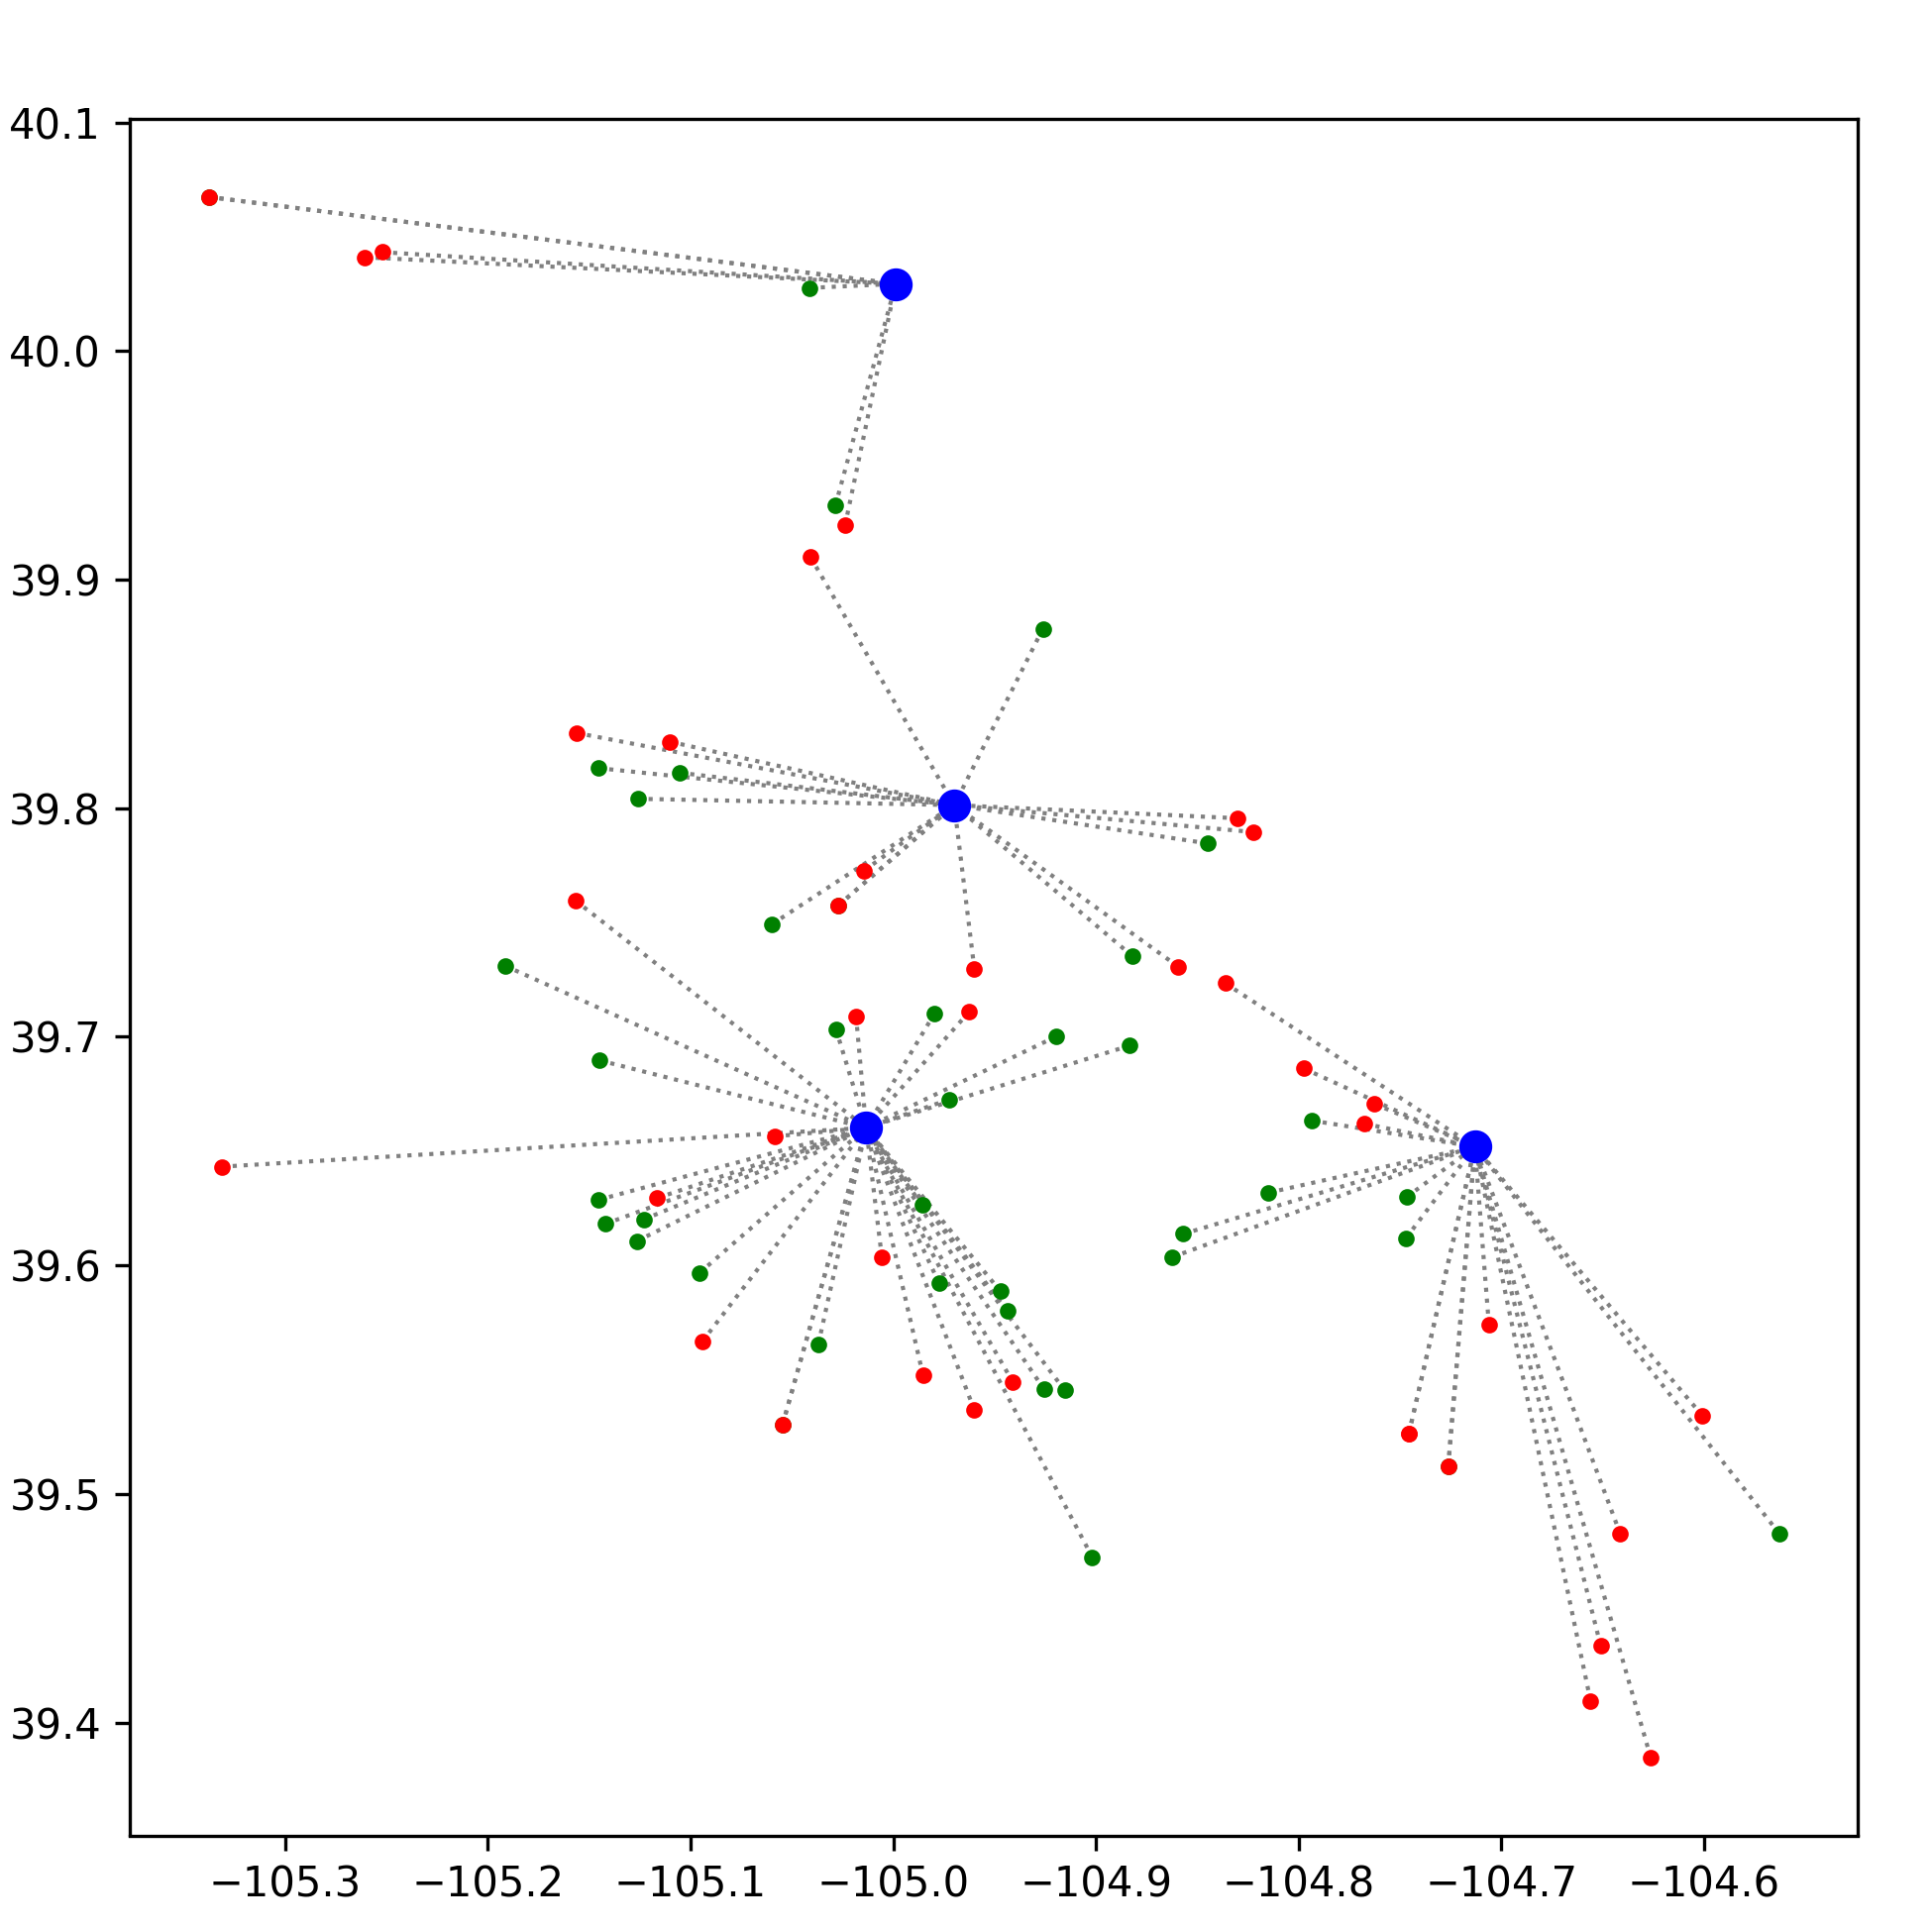
\includegraphics[width=8cm]{stars.png}\\
Blue dots are storage yards, green dots are pickups, red dots are deliveries.\\
  Figures made in matplotlib\cite{matplotlib}
\end{center}

\subsection{Triangles}
Since the problem doesn't actually consist solely of switches it is necessary to
expand the star solution to include pickups and drop-offs. This provides a route of landfill, drop-off, pick-up, landfill for a driver, creating a triangle. These triangle routes allow for further optimization as long as the optimal triangles are chosen.

\begin{center}
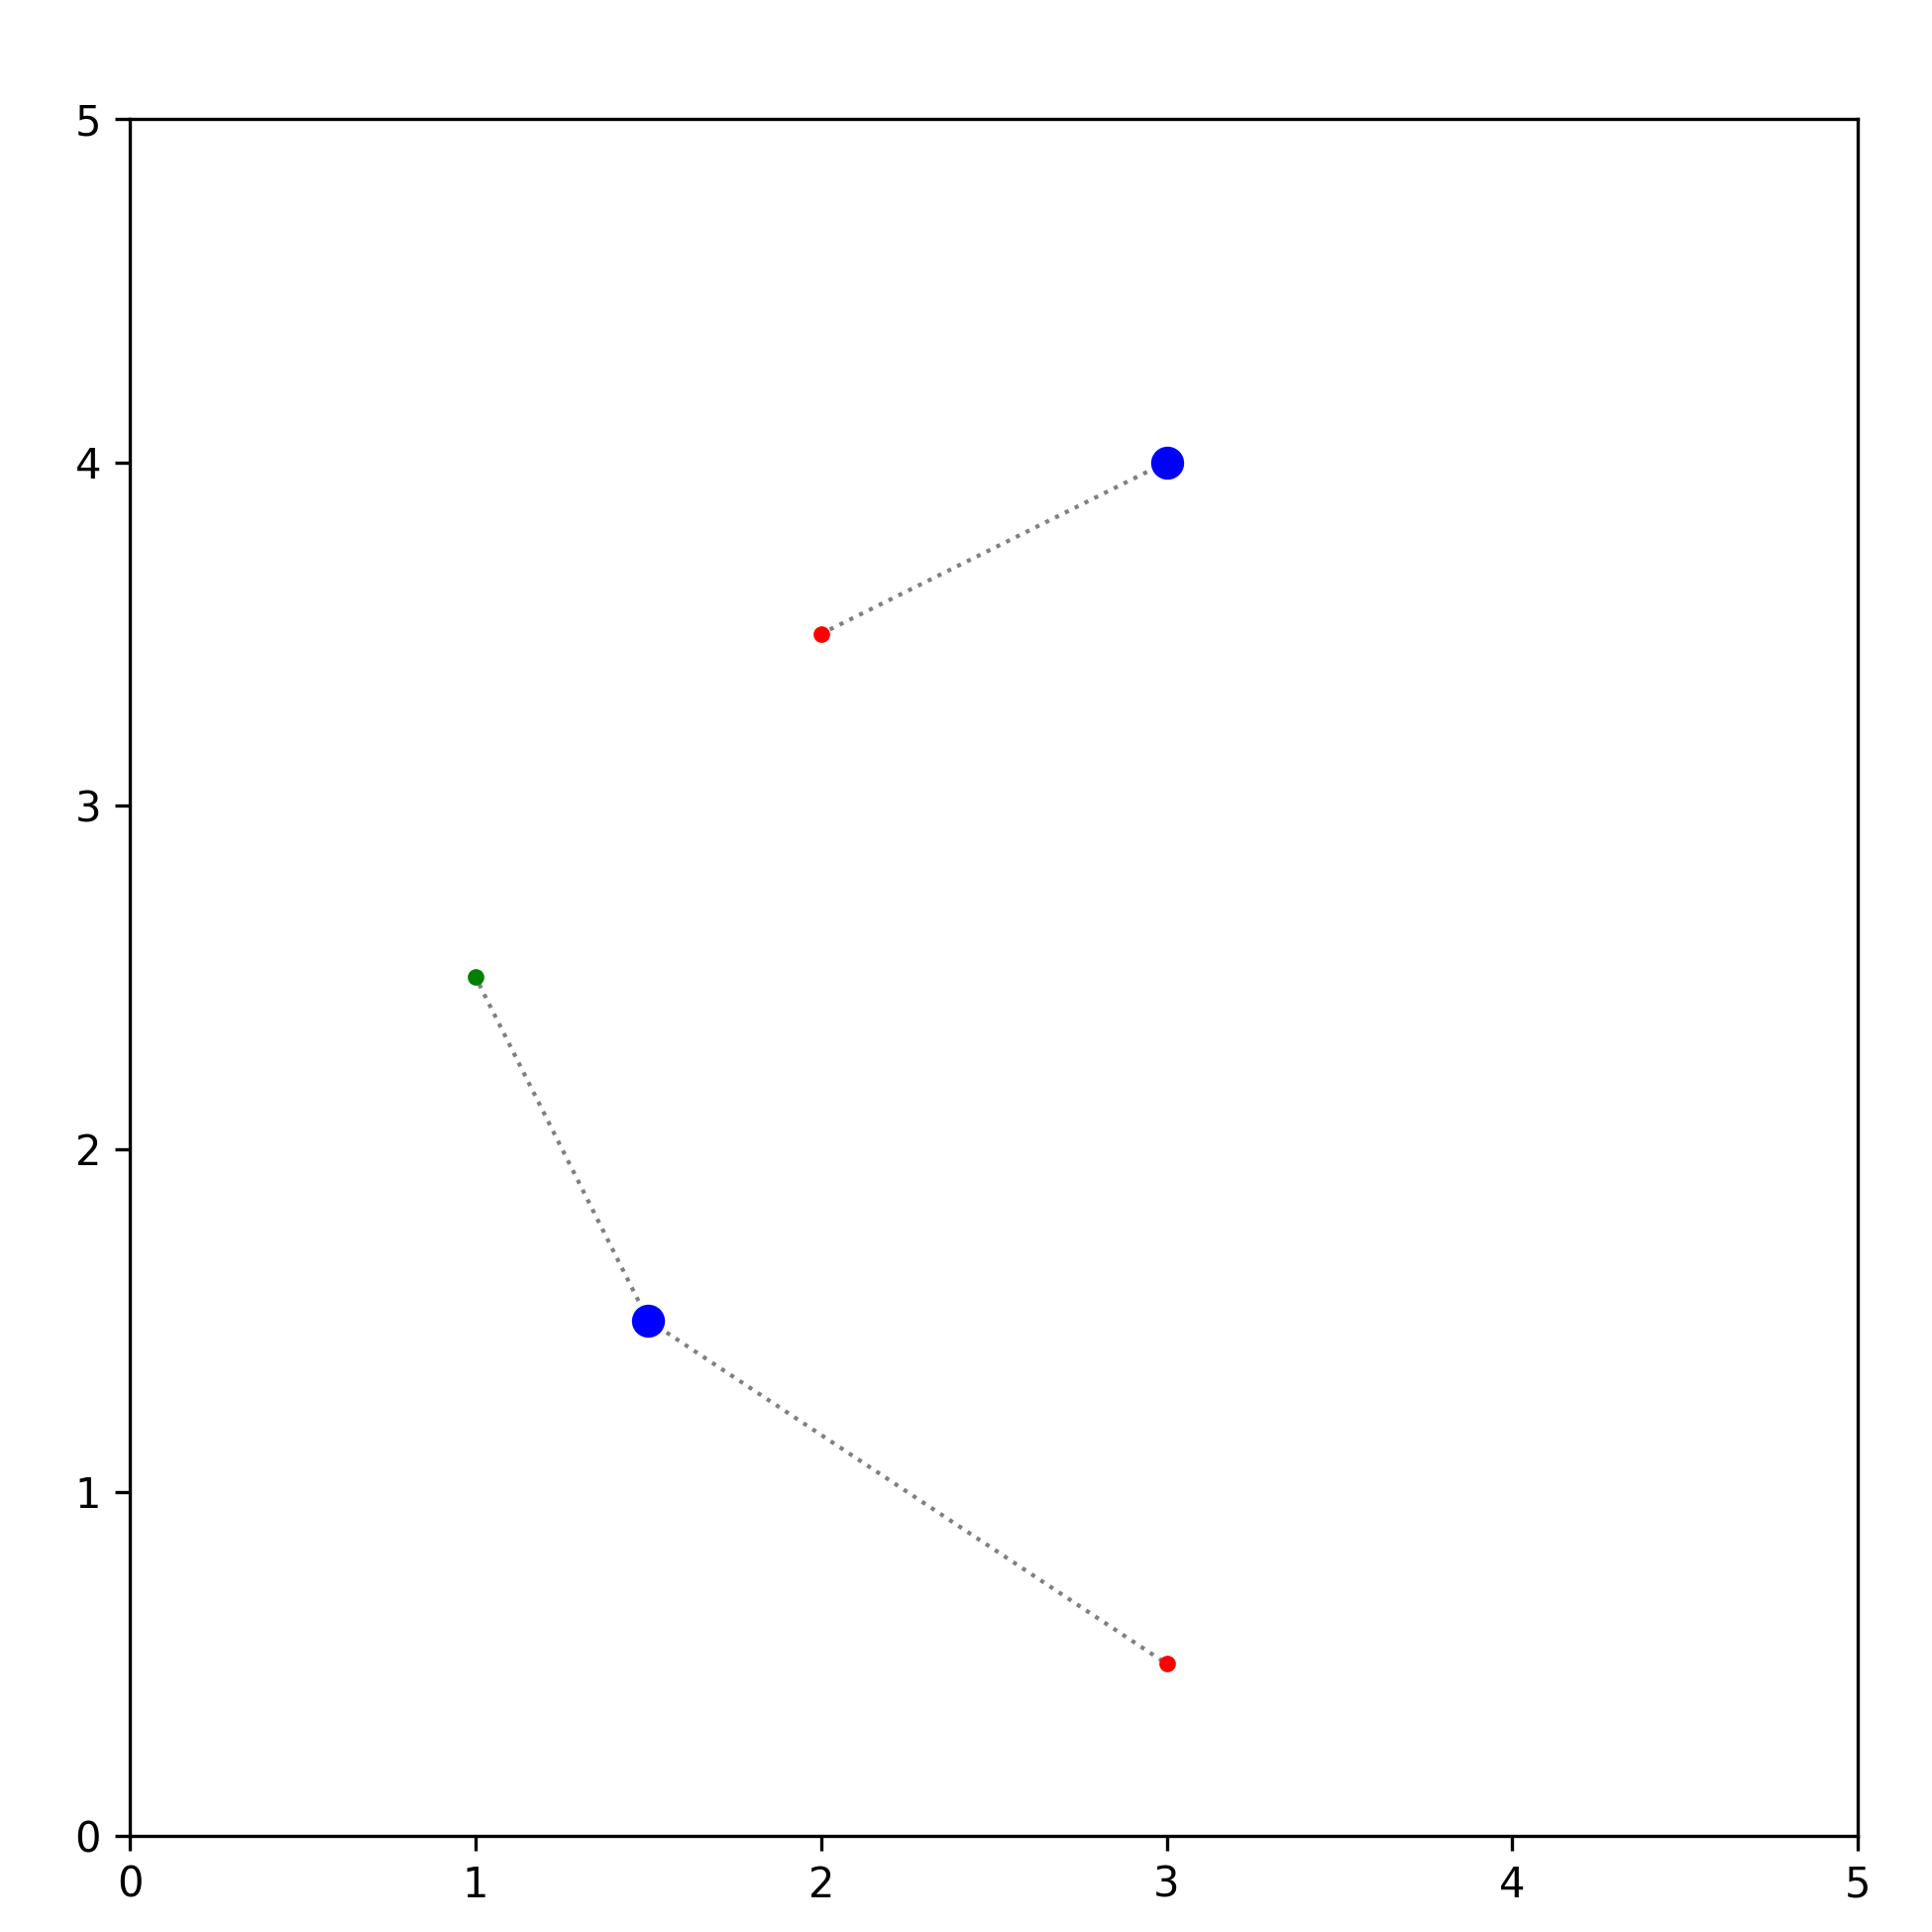
\includegraphics[width=5cm]{small_ex_star.png}\\
  Small example stars\\
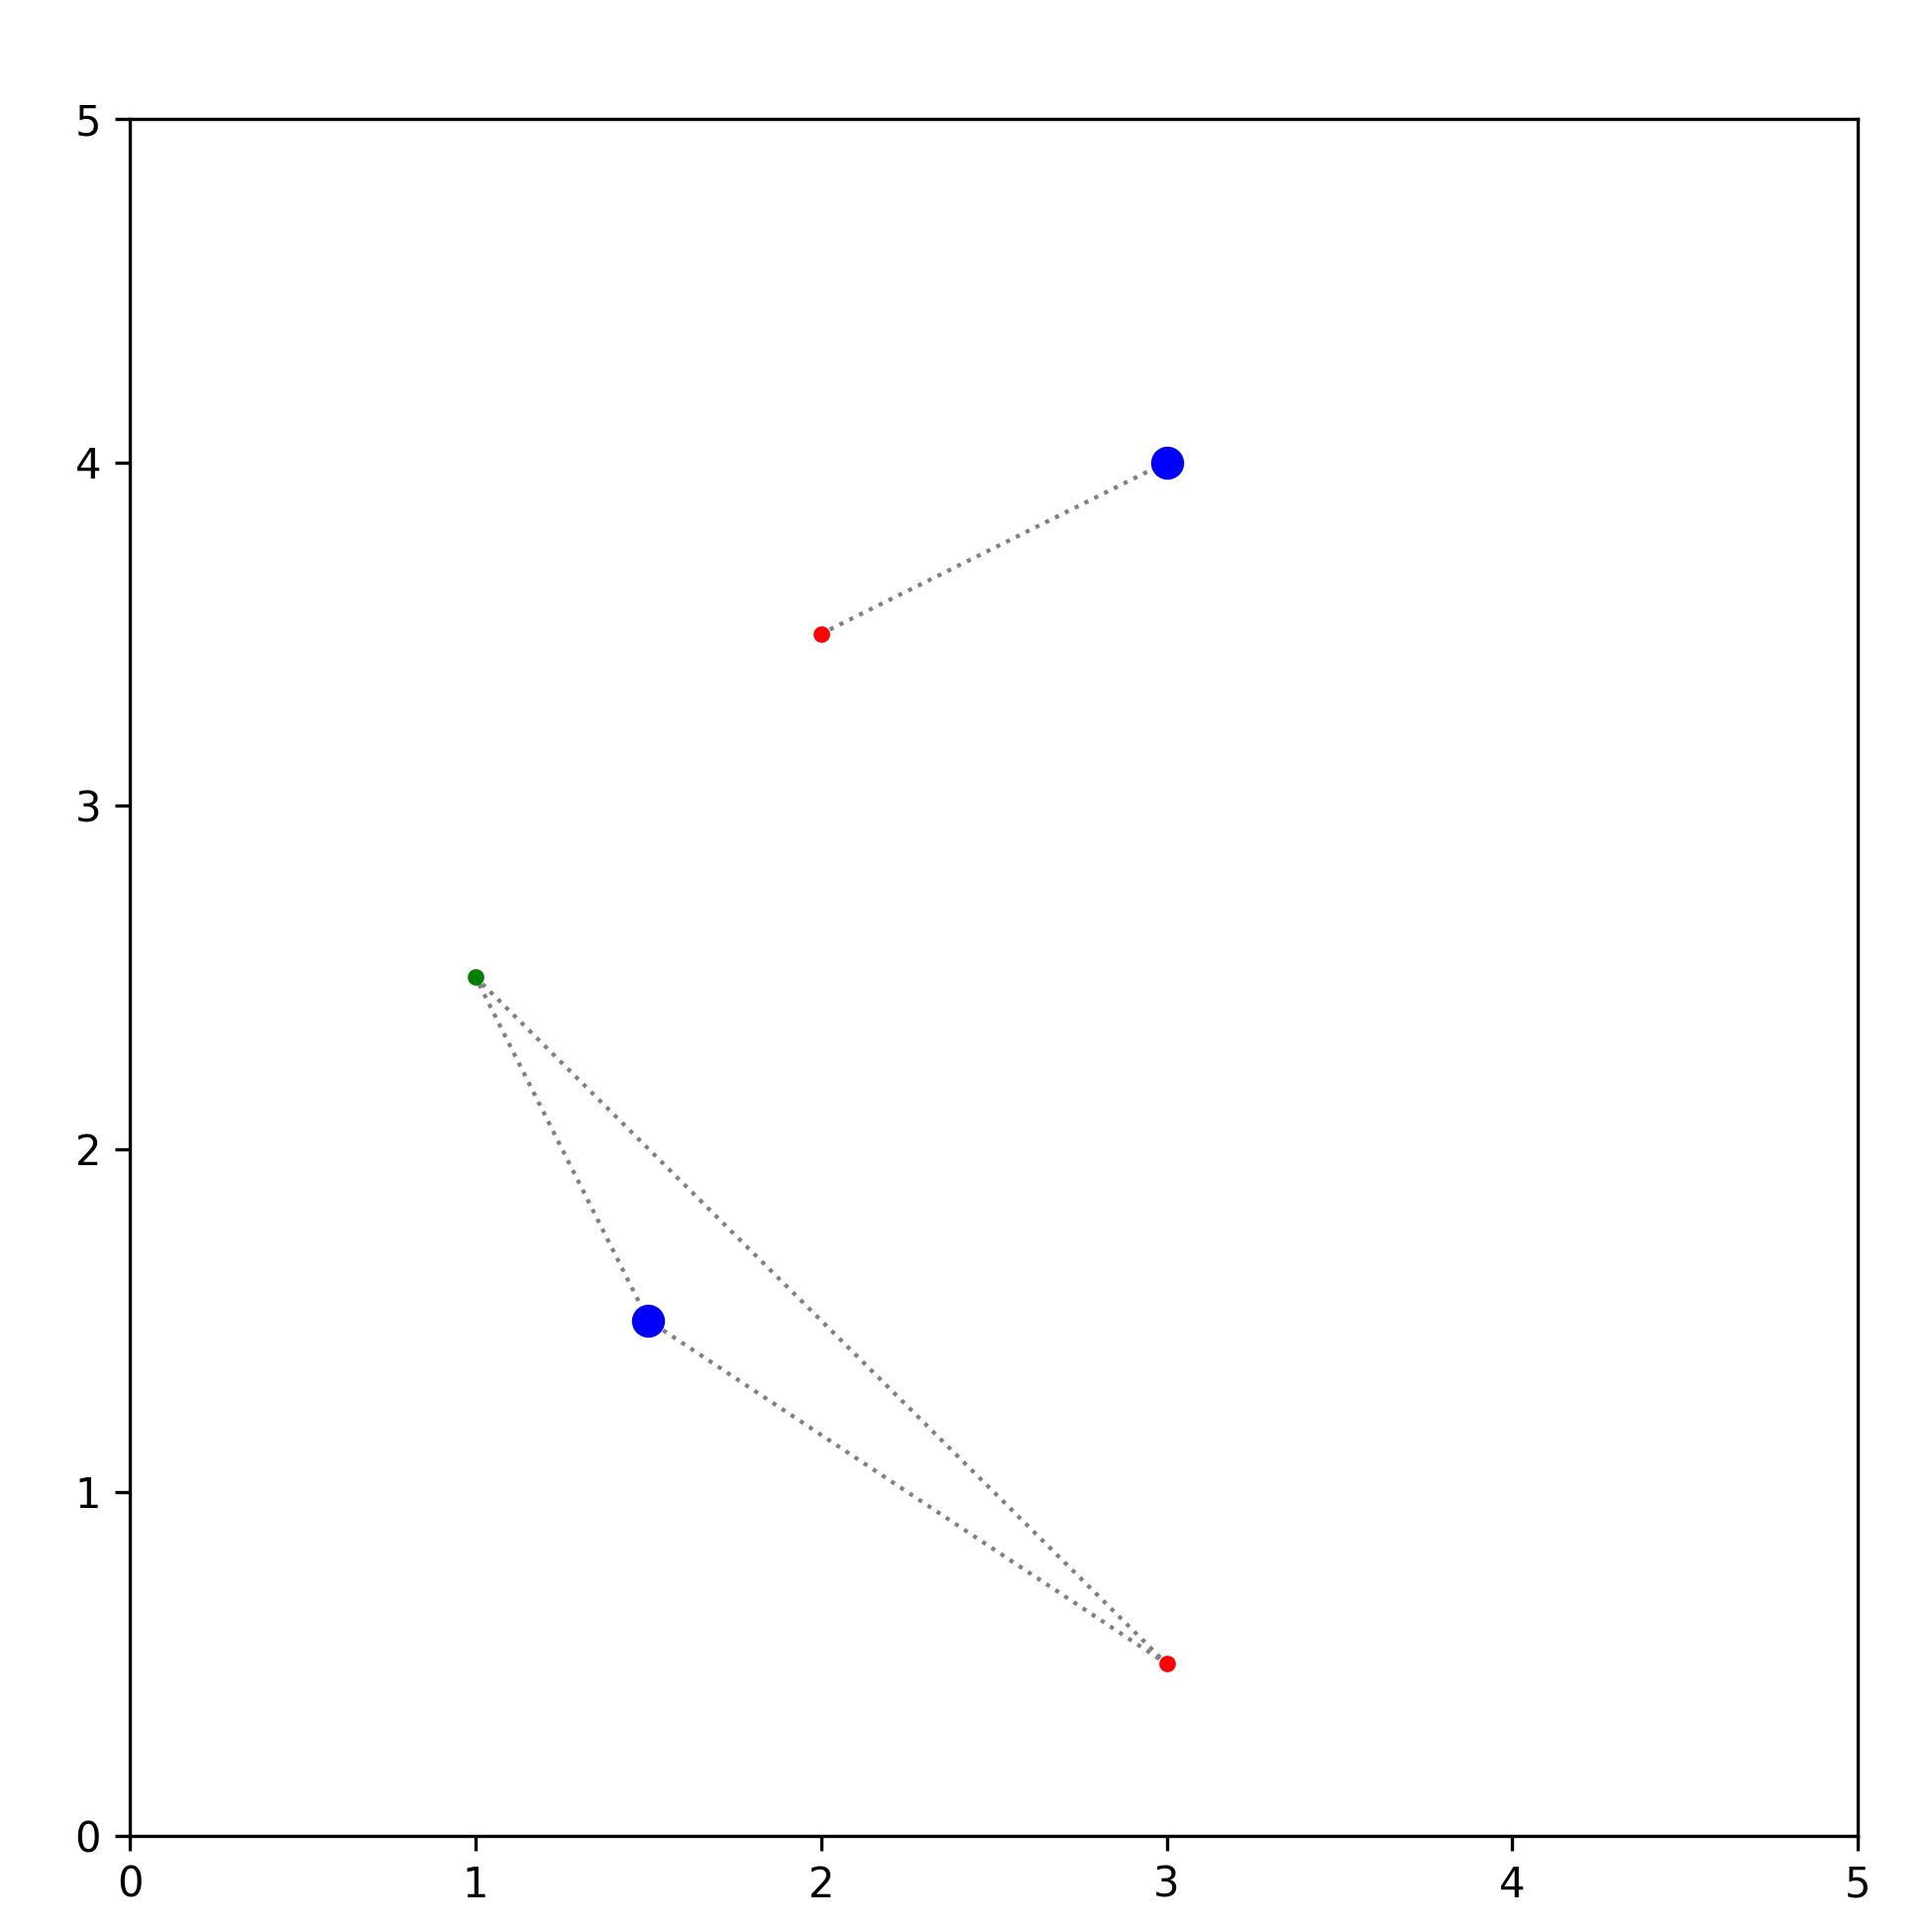
\includegraphics[width=5cm]{small_ex_ok.png}\qquad
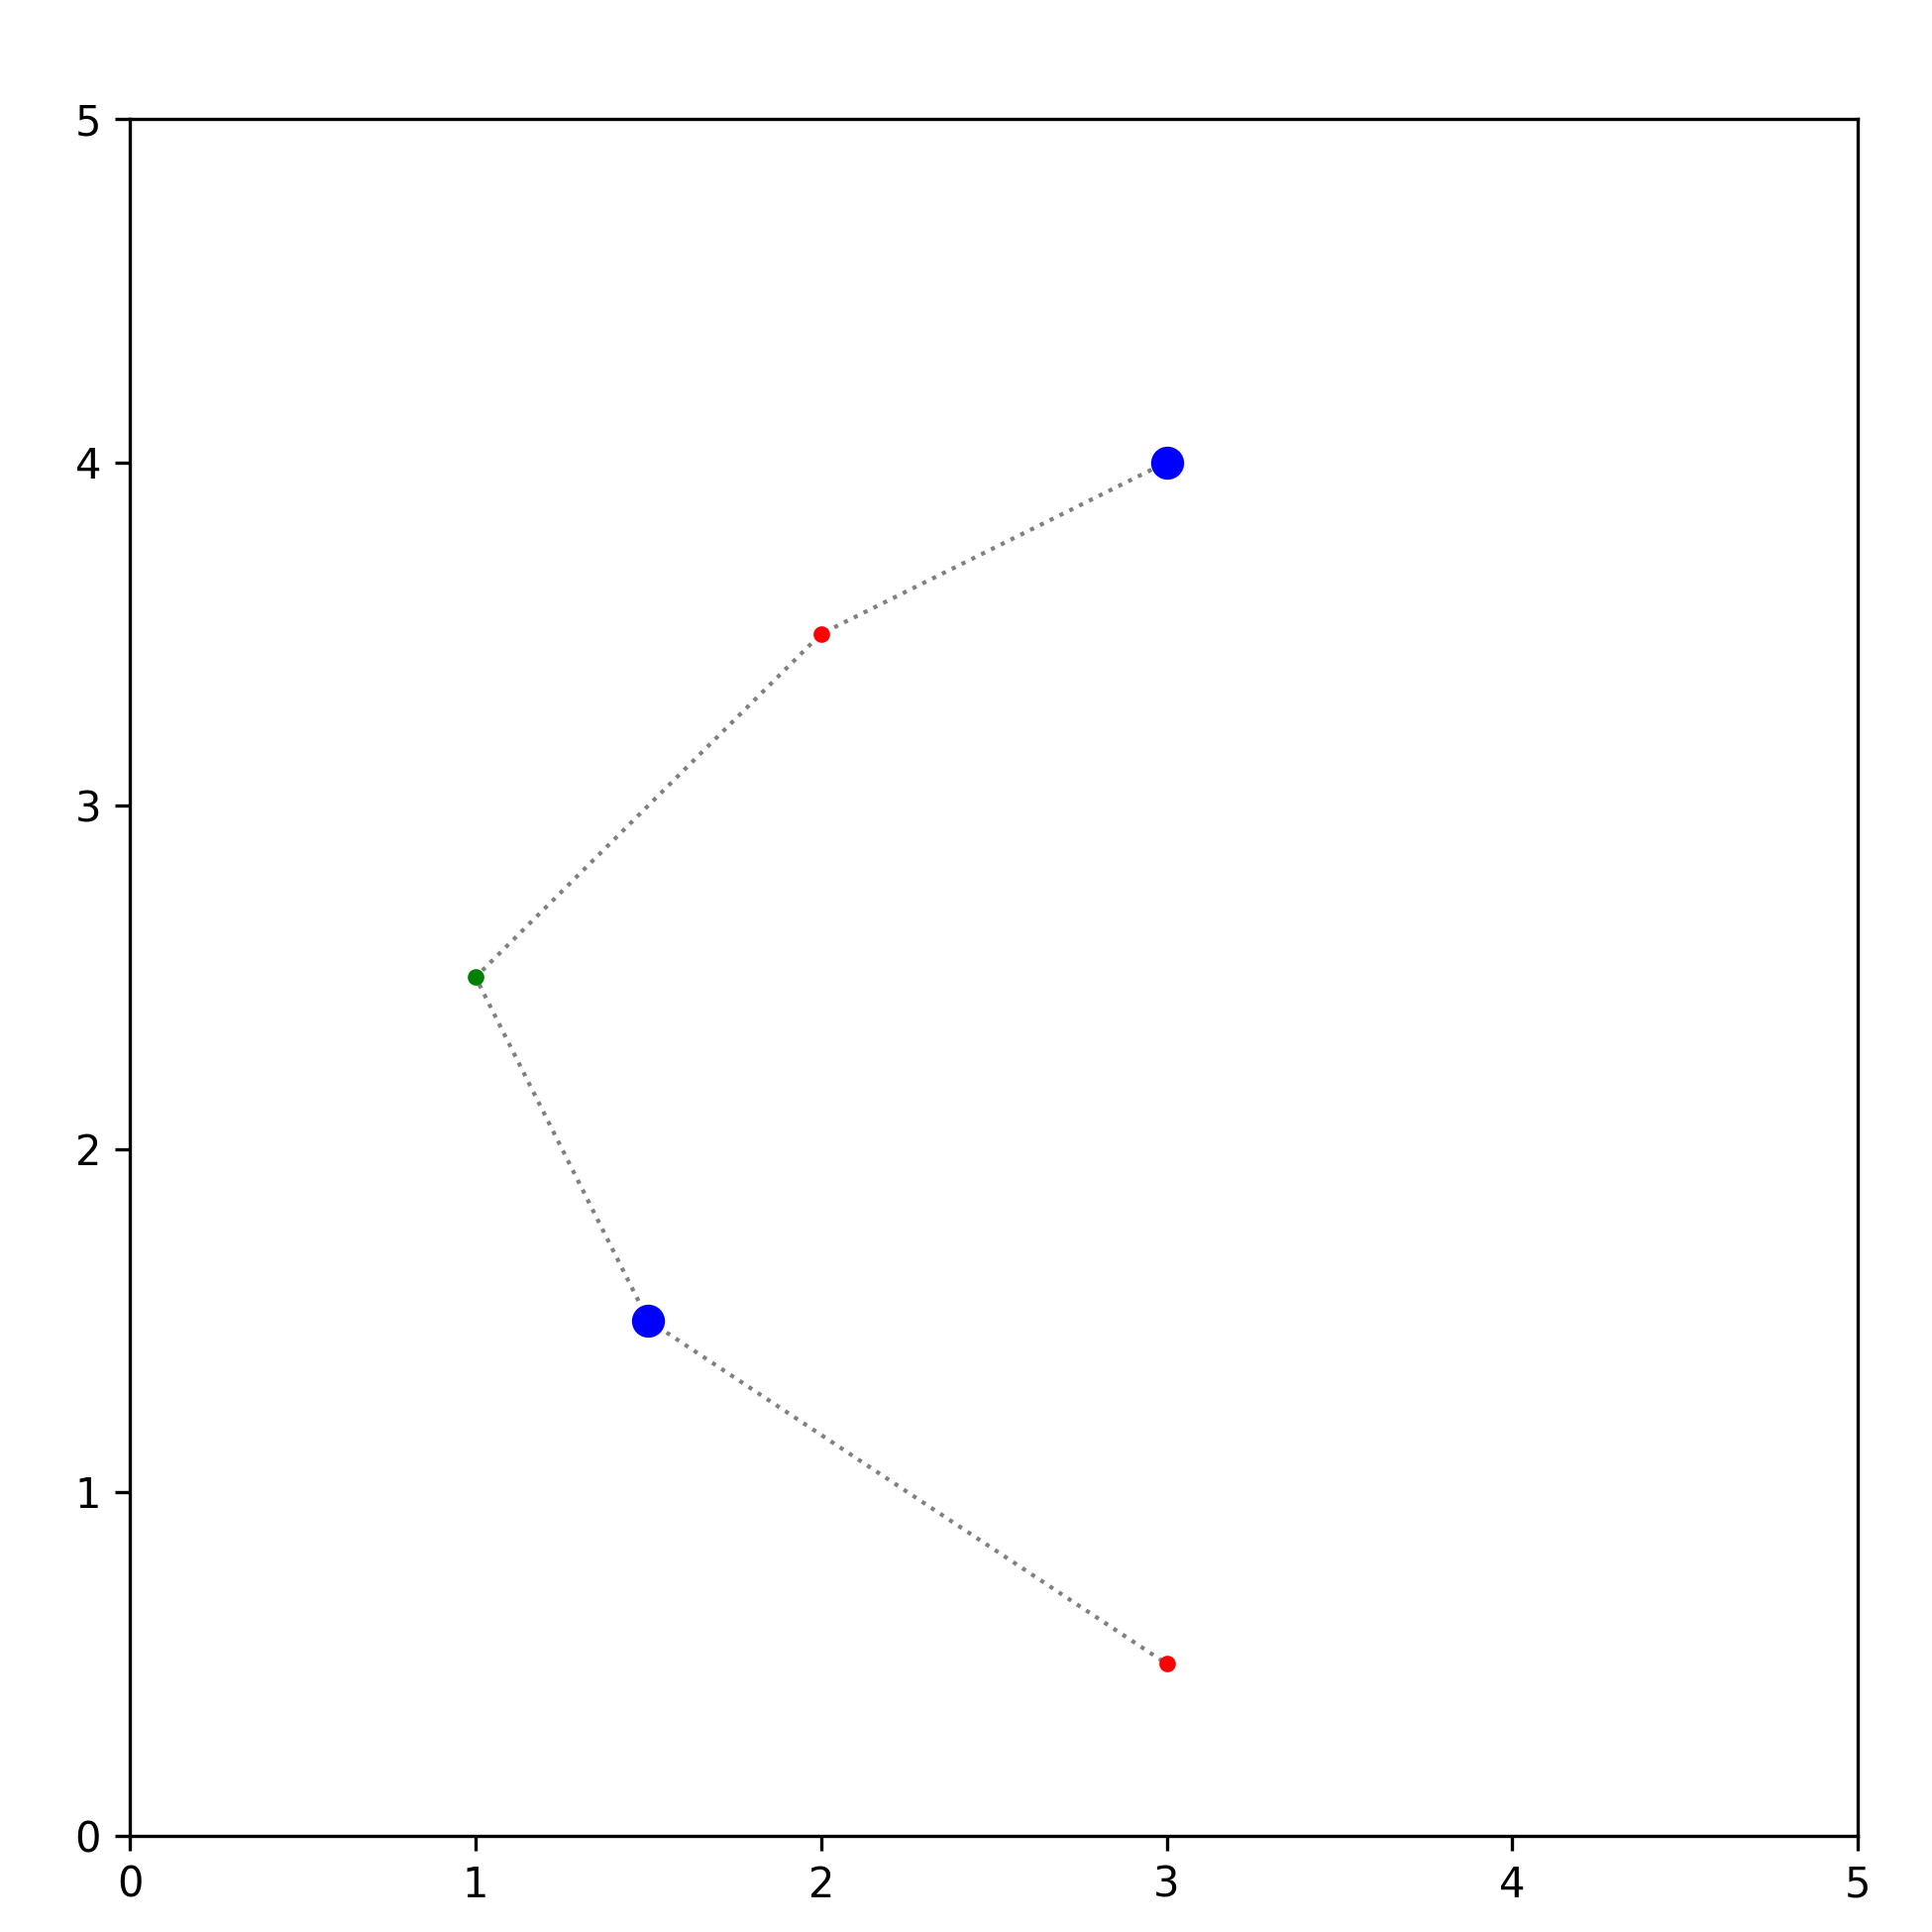
\includegraphics[width=5cm]{small_ex_best.png}\\
  On the left we have already done better than the star example above, however,
  the configuration on the right requires less driving, and moves a driver from
  one storage yard's zone to another.
\end{center}

Some triangles are better than others, so what we want is the best \emph{set} of
triangles, those which minimize the total amount of driving over the entire map.
This type of problem has been studied before, it is known as the Assignment
Problem\cite{hungarian}, and the people who studied it made an extremely efficient way
to solve it optimally (no approximations!), known today as the Hungarian
Algorithm\cite{hungarian}. We make use of an implementation of that
algorithm\cite{munkres} to calculate that optimal triangle setup, keeping in mind
compatibility between pickups and deliveries.

In order to use the algorithm, we need to associate a ``weight" to every pair.
The algorithm generates the best pairs based on that weight. To calculate these
weights, we take the difference between what the pair would cost individually,
as a star, and what they would cost together as a triangle. Minimizing this
maximizes the ``benefit" of the triangles over the stars, which is exactly what
we want.

We allow for pairs to cross between landfill zones, that is, the delivery has
one closest storage yard and the pickup can have a different closest storage
yard. In a matching where this is allowed, the result is almost always better than
restricting pairs to the same zone. One unfortunate consequence is that the
name ``triangle" becomes less intuitive.

\begin{center}
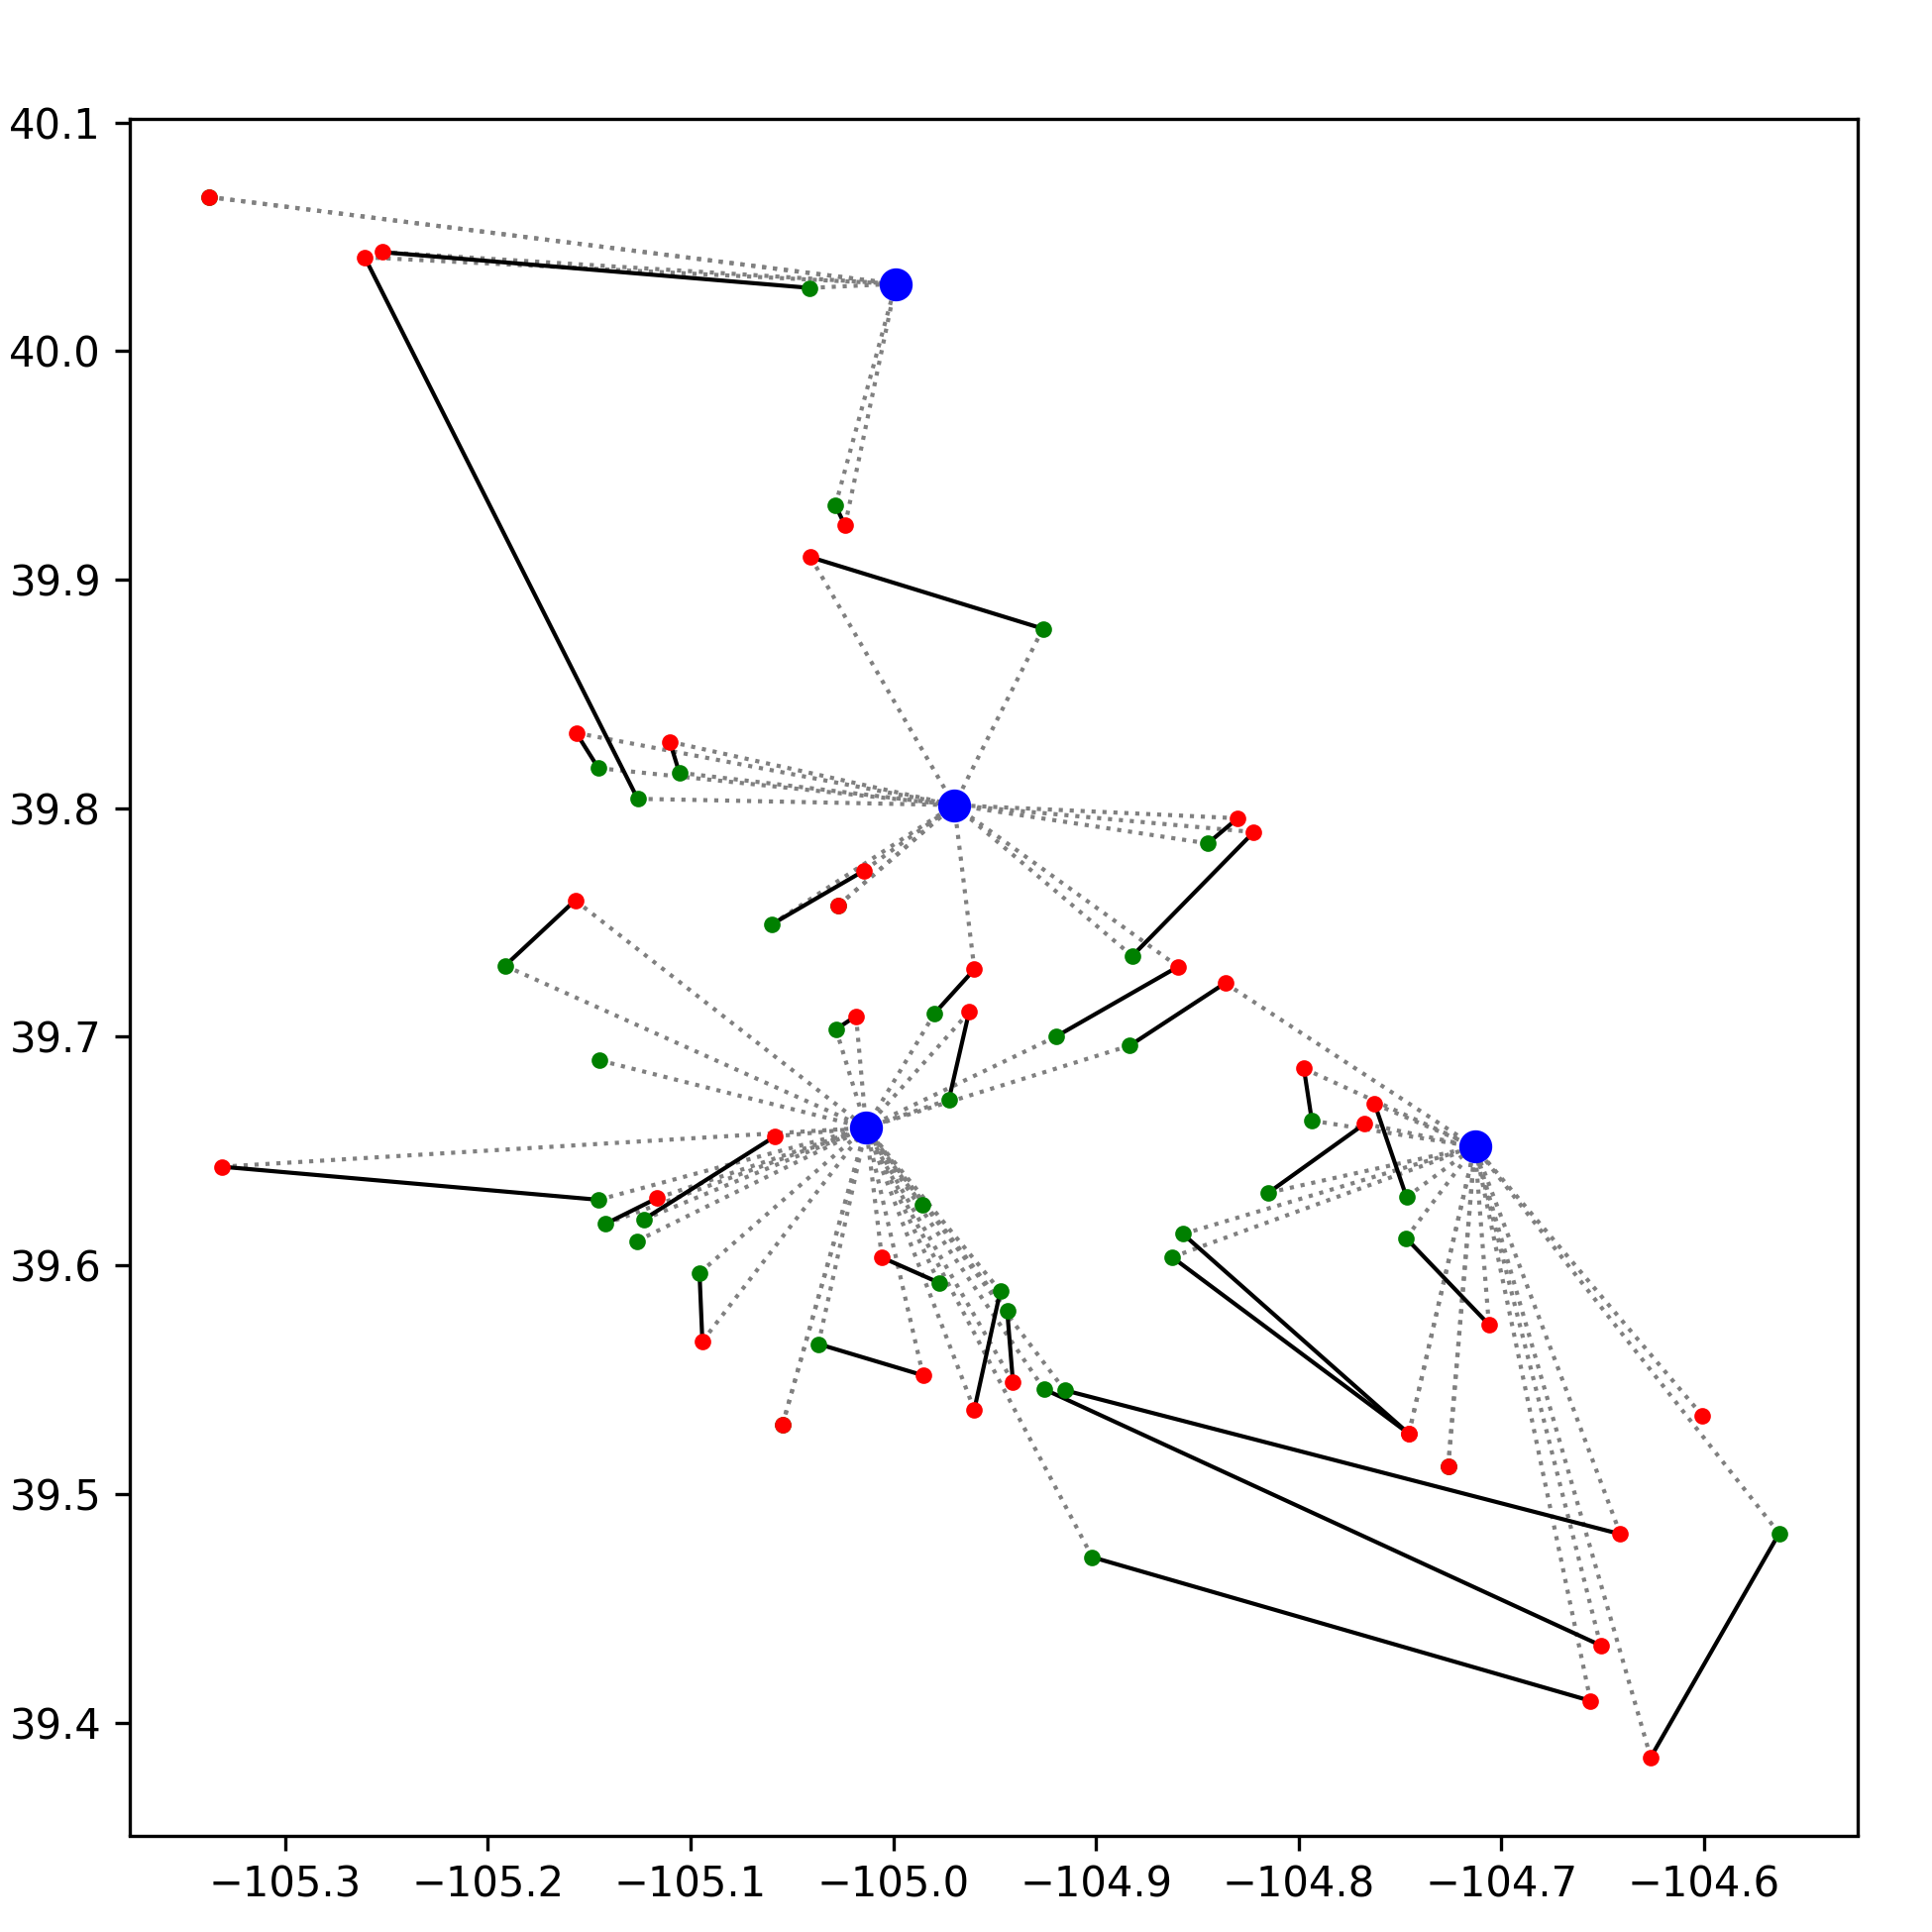
\includegraphics[width=8cm]{triangles.png}\\
Deliveries and Pickups matched from real data. 
\end{center}


\subsection{Route Building}
Now that we have matched up deliveries and pickups optimally, we need to
allocate the jobs to the drivers in a reasonable way. For this, there are three
considerations, how do we move drivers between storage yard zones? (transitions), how do we satisfy truck and time of day constraints? And how do we manage the supply of cans among the storage yards?

\subsubsection{Transitions}
In order to determine each transition, we calculate $\min (RN_i - RT_i)$ for $i=0$ to $i=n$ where $RN$ is the route cost normally, $RT$ is the cost of doing the transition, and $n$ is the number of job pairs that have not been assigned to a driver. In the case where pairs are constrained $\min(RN_i - RT_i)$ will always be positive since one of the two endpoints is no longer to the closest landfill. However in the case where pairs are non-constrained and can be made between zones the cost of doing a job pair normally can be greater than the cost of doing a transition since the pair can have different landfills that are closest. 

\subsubsection{Non Transition Routes}
Non-transition routes are first assigned to fulfill constraints, second to match the size of the can the driver just picked to the size of can to be delivered next and are assigned in descending order based on their distance to the main hub of the company.

\subsubsection{Truck and Time Constraints}
Two constraints that need to be considered are the time constraint and the truck size constraint. Customers may request a delivery in specifically the AM or PM hours of the day. In order to
deal with this constraint, routes identified as such are assigned with priority when a driver’s schedule is within the time period. In addition, some trucks are restricted as to where they can deliver cans. This constraint is resolved by identifying routes that require a specific truck and assigning the first driver that truck with a special schedule that services all routes with the constraint and then performs as a regular driver within the zone they end in. If more Truck constraints exist or the first driver did not complete all of the constraints for the size he was assigned another driver will be assigned in the same manner until this is resolved

\subsubsection{Can Supply Management}
A final issue considered is the supply of cans at a given depot. There are two types of can deficits that must be dealt with. First are hard can container deficits which occurs when there are more cans that need to leave the storage location than will be returned plus the initial stock on a given day. These can be resolved in two stages. The first stage is for a deficit of size up to the number of drivers that will start their day driving to the zone with a deficit. In this stage the calculation for transitioning will be altered to only consider routes with a pickup of the appropriate size can outside the zone with the deficit. In the second stage where the problem cannot be resolved in the initial stage the first driver assigned to the area will be assigned special transitions that both originate and end in the deficit zone, but which leave in order to go to a pickup of the size of the can with a deficit.
A soft can deficit, which means that the number of returns plus the initial stock of cans at a depot is at least as large as the number of cans of a particular size that need to be delivered. This can still be an issue if too many deliveries happen before the pickups for a particular size of can. Even where returns plus the initial stock are at least as large as the number of cans of a particular size, a problem may occur if too many deliveries happen before the pickups for a particular size of can. To resolve this the draft schedule is simulated through the day and where conflict arises a swap will be made to fix the problem with priority given to swapping within the same driver’s schedule. Due to how our solution works these swaps will not affect the efficiency. When considering whether an issue exists other driver’s schedules will be considered to be at a time less than the current simulated time by some amount of minutes L to account for potential differences due to delays.

\subsection{Recap}
The algorithm for assigning the full schedule are as follows:
\begin{enumerate}
\item Receive data for the day and process it into the program.
\item Create pairs with Hungarian algorithm.
\item Assign driver to resolve truck size constraint.
\item Transition to the farthest zone that requires the truck resolving a hard can deficit if applicable.
\item Service all routes within the zone that require the truck and return to step 2 if more applicable routes exist in other zones.
\item Finish route as per a normal driver and return to 1 if other truck size constraints exist.
\item Assign driver to farthest zone with routes.
\item Transition to the zone.
\item If applicable resolve hard can deficits.
\item Assign remaining routes by prioritizing AM/PM constraints, then routes where the delivery can size is the same as the pickup from the prior pair of routes, and finally distance to the main hub.
\item If there are no more routes in the zone transition to the next zone and return to step 8.
\item If the driver schedule is full including the transition back to the main hub transition back to the main hub and return to step 7 with a new driver.
\item Iterate through the day to resolve any soft can deficits making swaps as needed.
\item Output schedules.
\end{enumerate}

\section{Results} \label{grp1:results}
From an old schedule provided by the client, we ran our algorithm to see how it stacked up to the clients solution. In the following figures, each color is a driver's route.


\begin{center}
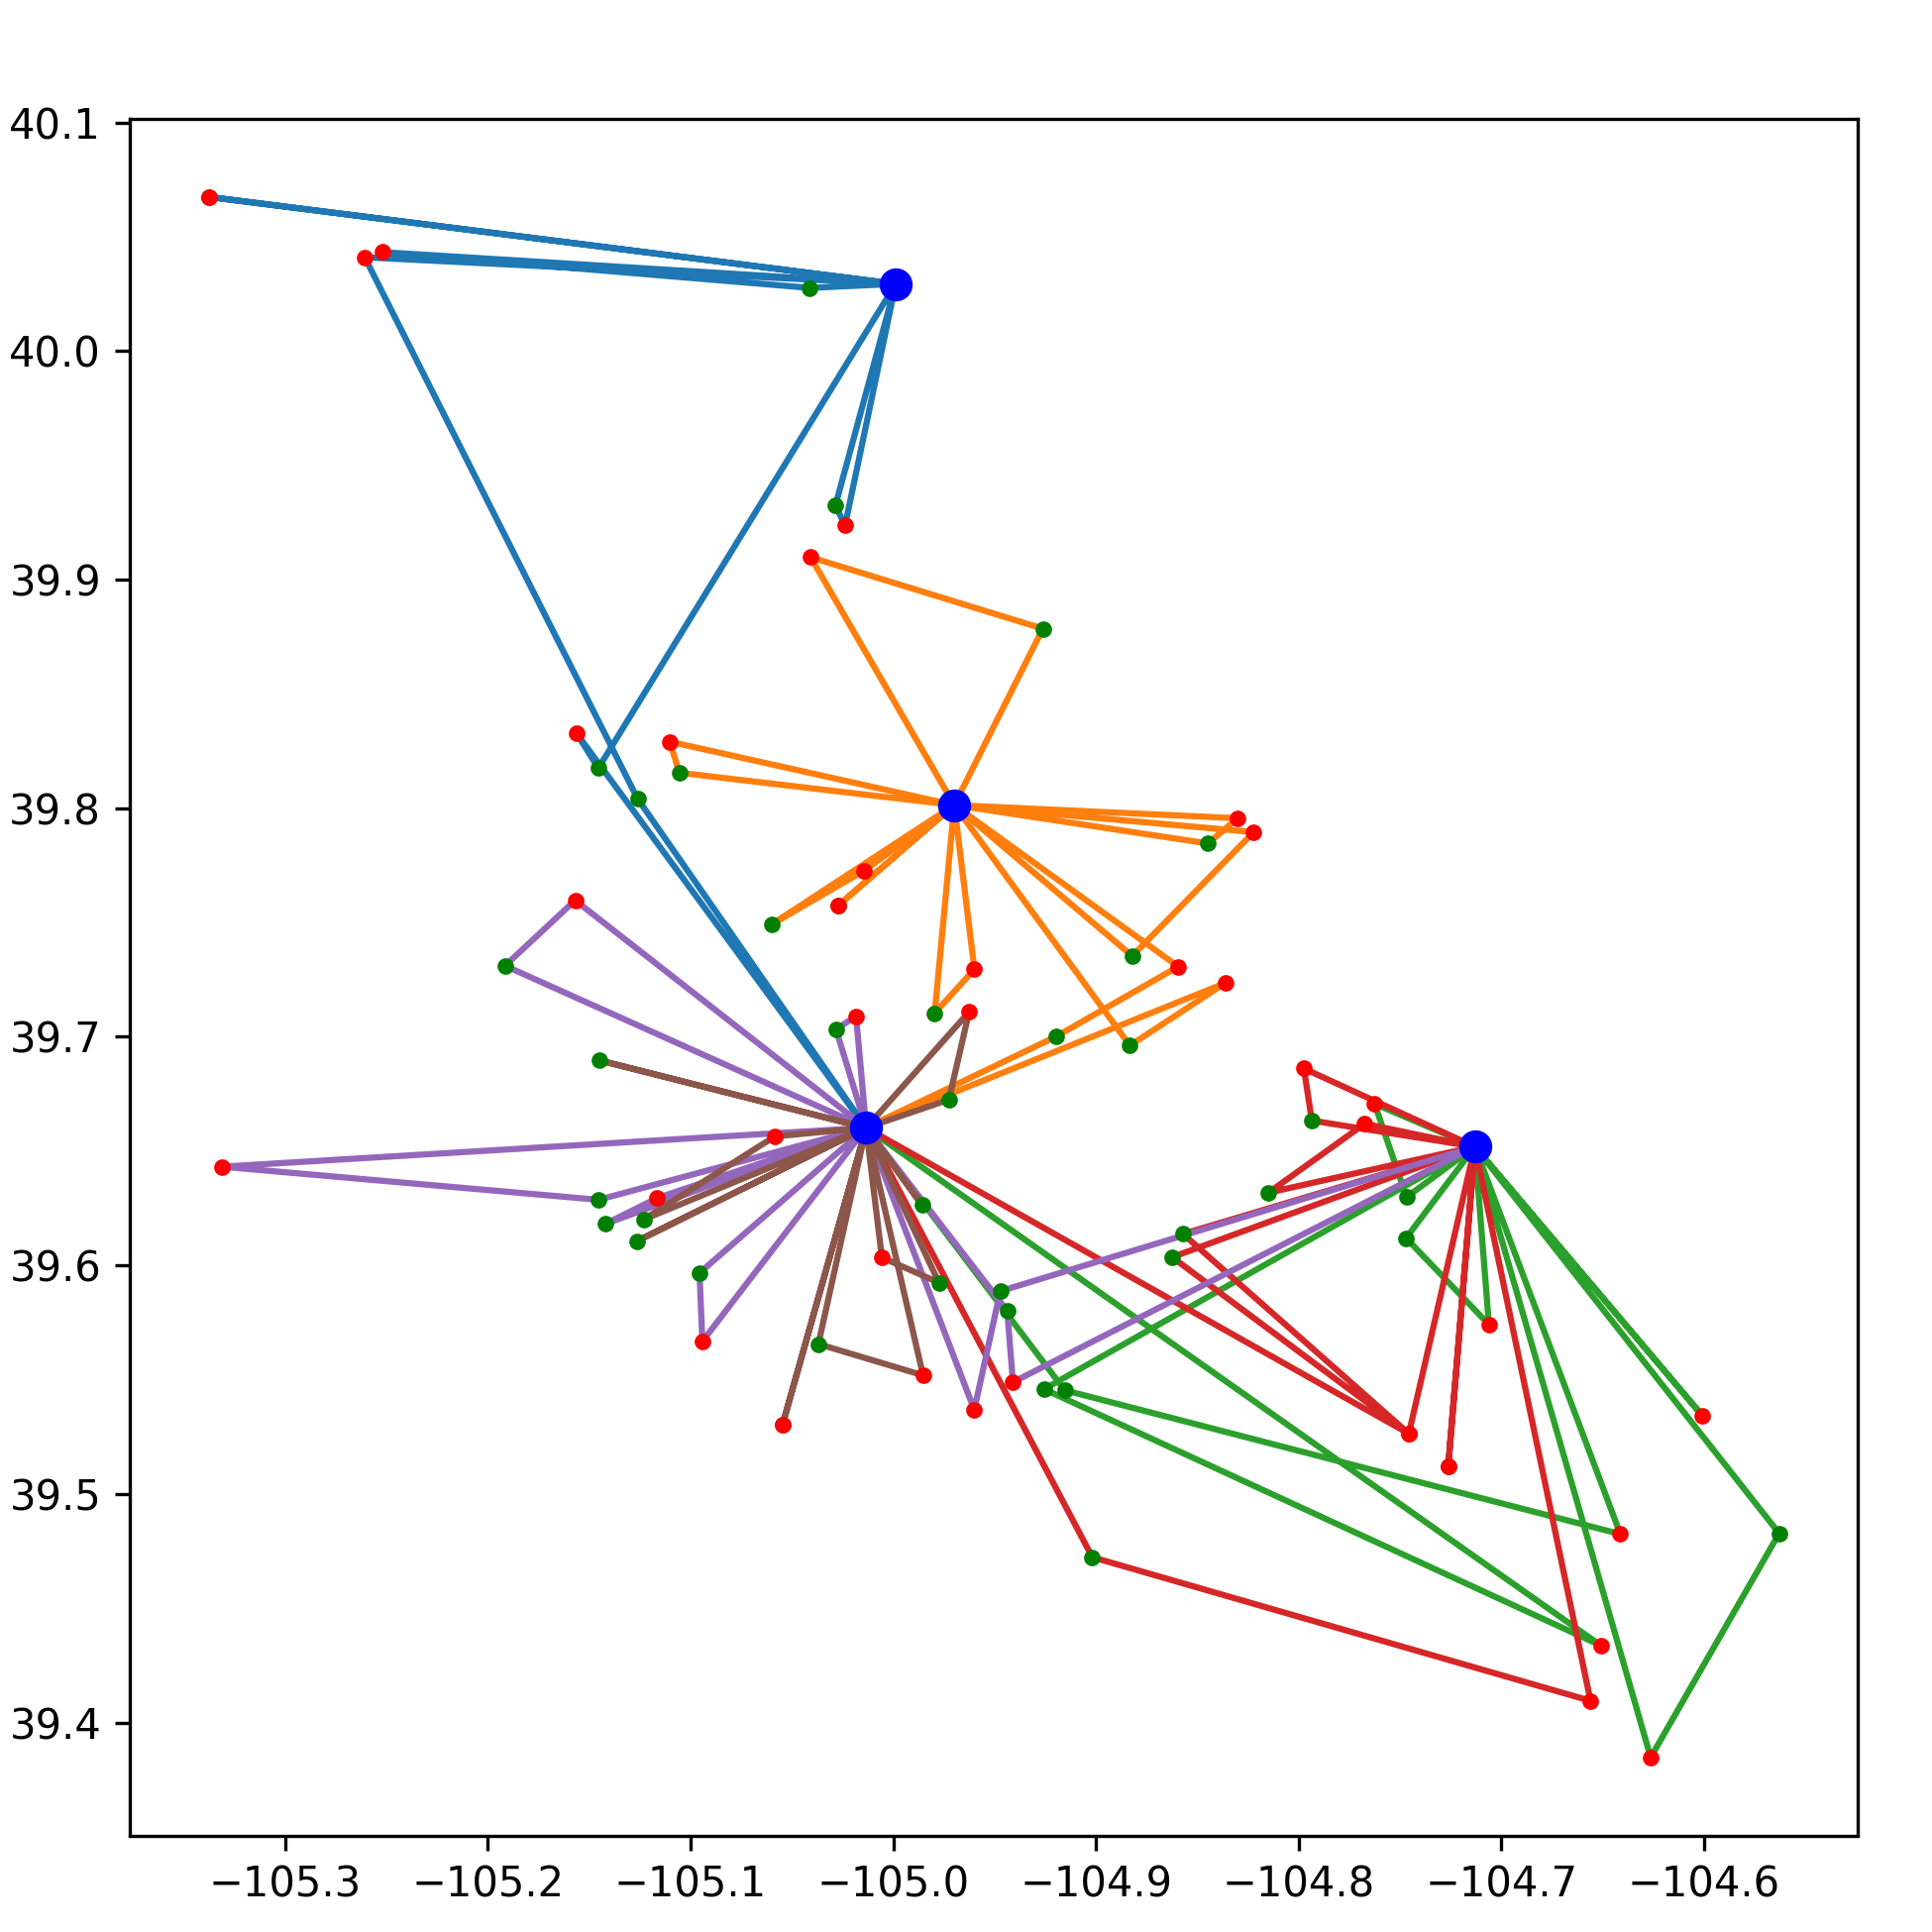
\includegraphics[width=8cm]{our_route.png}\\
	Routes generated by the algorithm. Total time spent driving:
  $1576$ minutes.
\end{center} 

\begin{center}
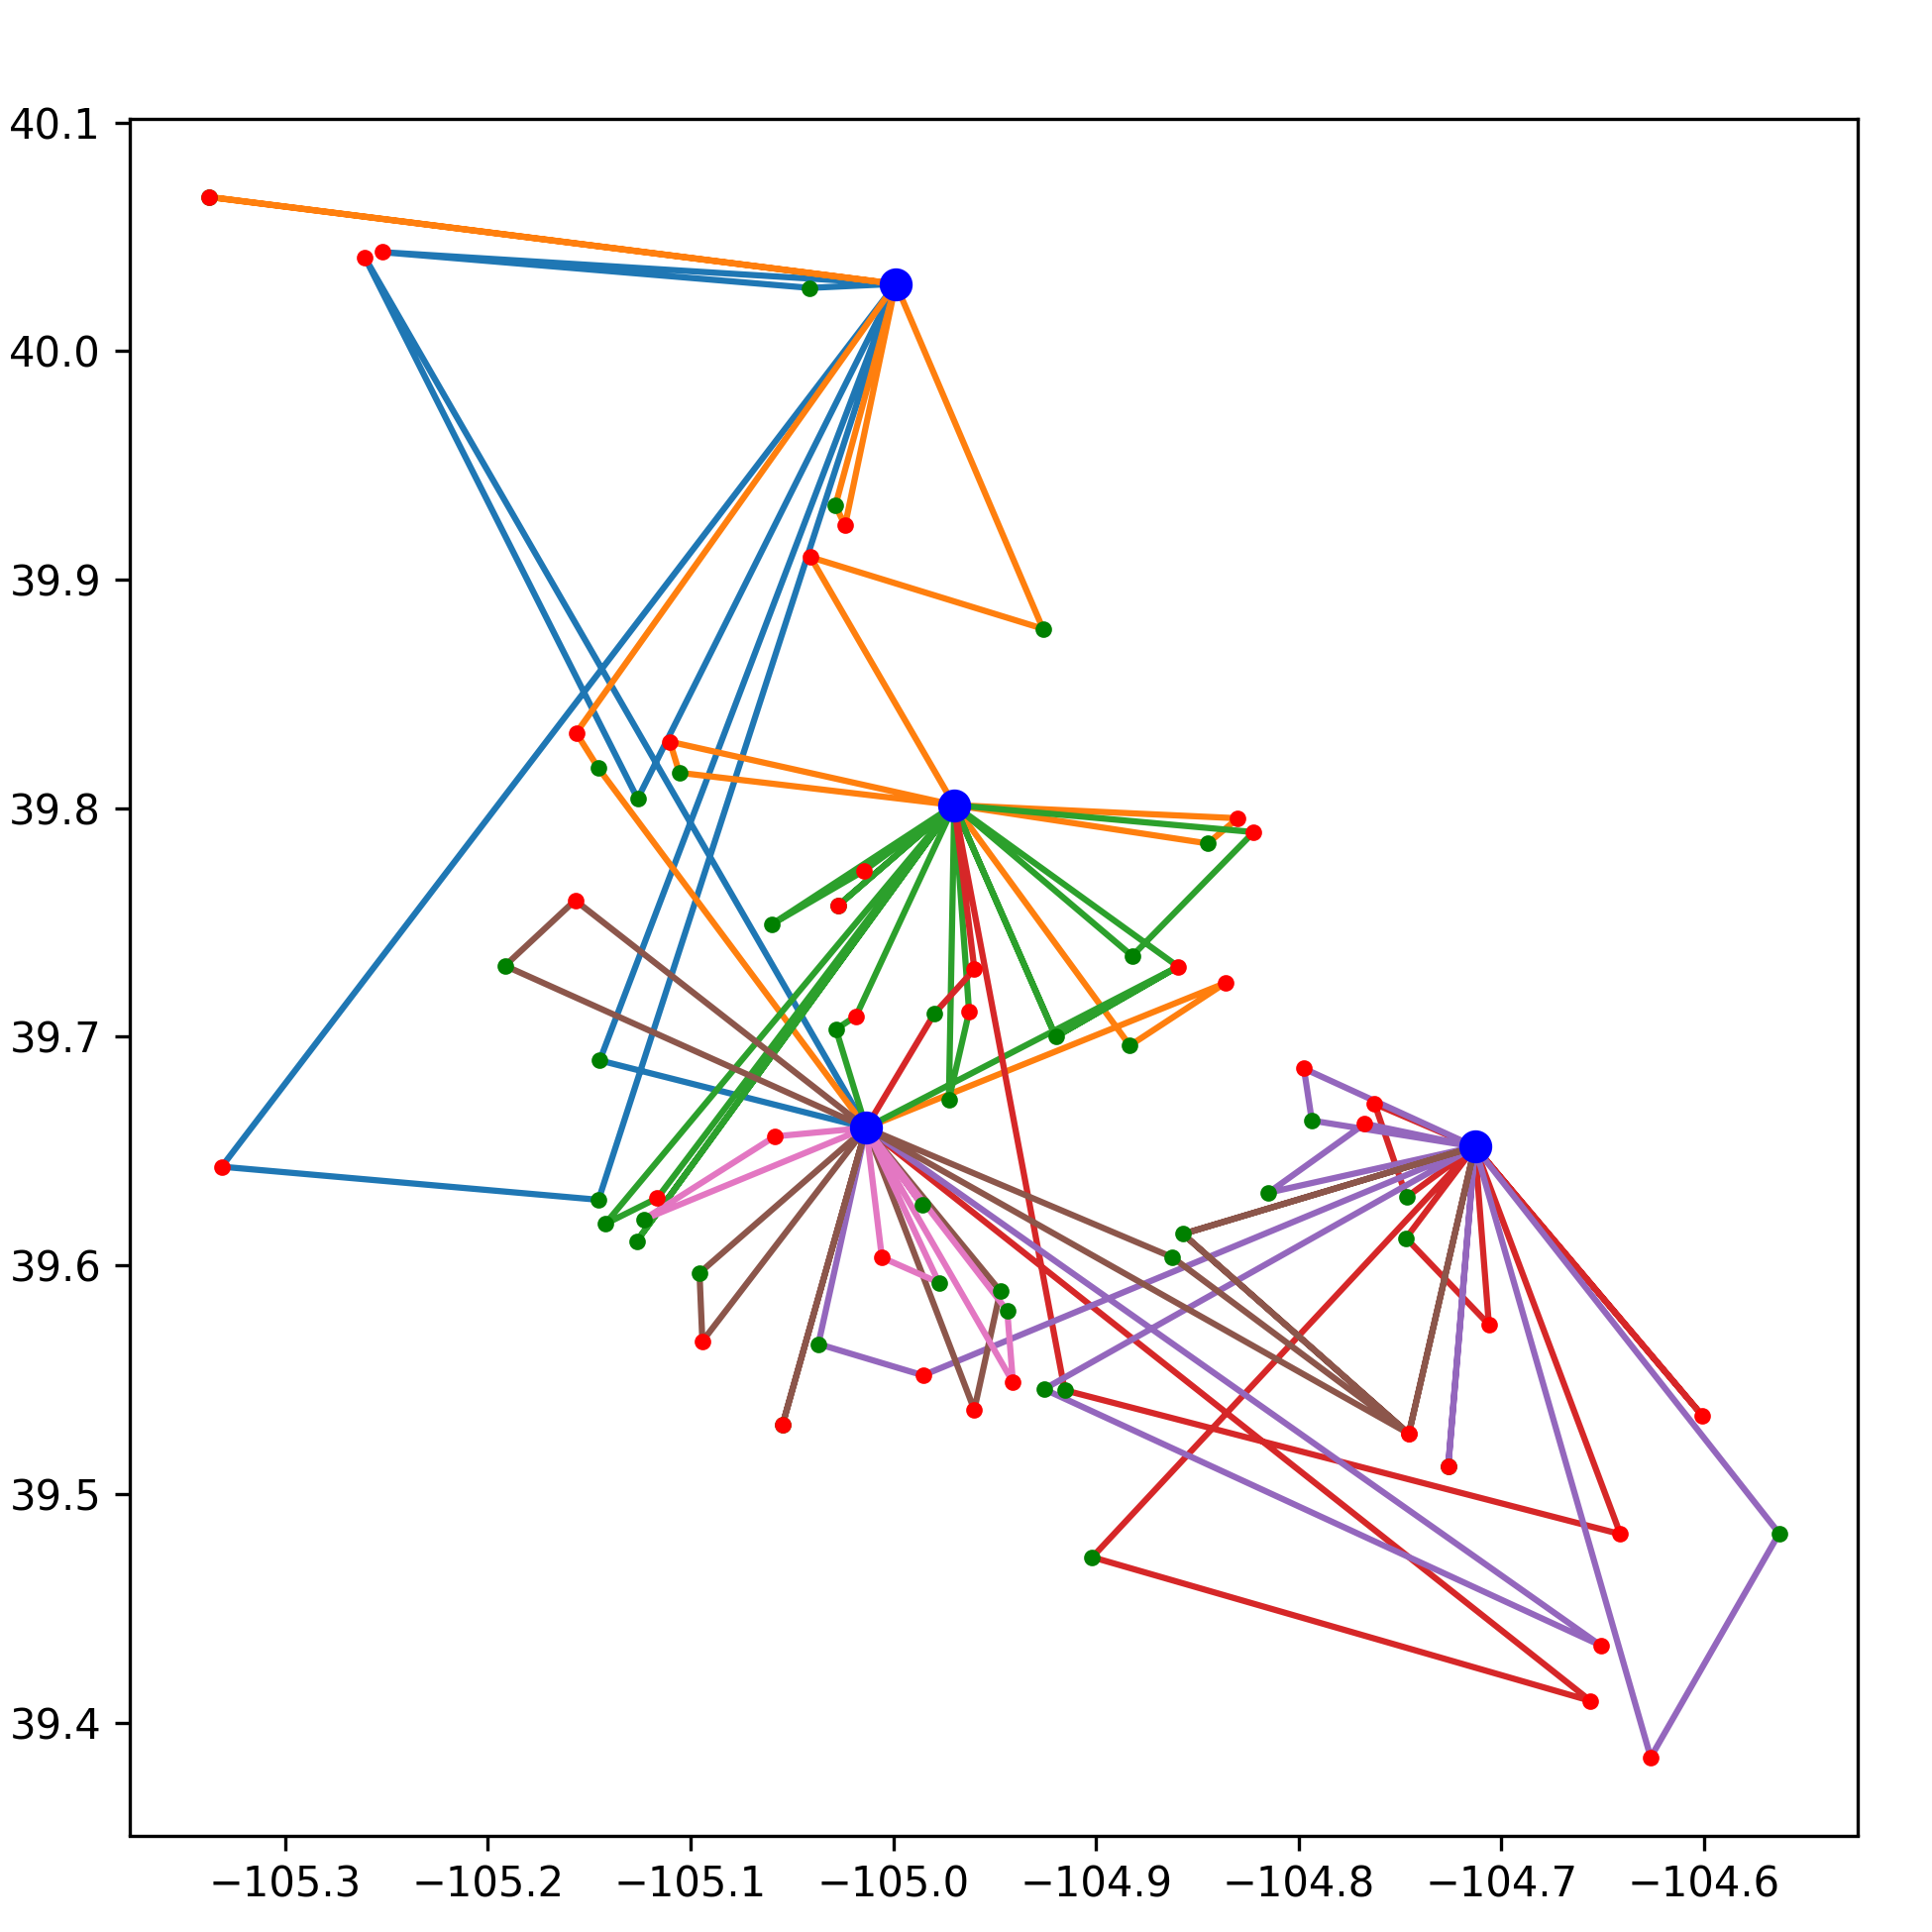
\includegraphics[width=8cm]{our_route_cans.png}\\
	Routes generated by the algorithm, including severe can
  restrictions. Total time spent driving: $1781$ minutes.
\end{center} 

\begin{center}
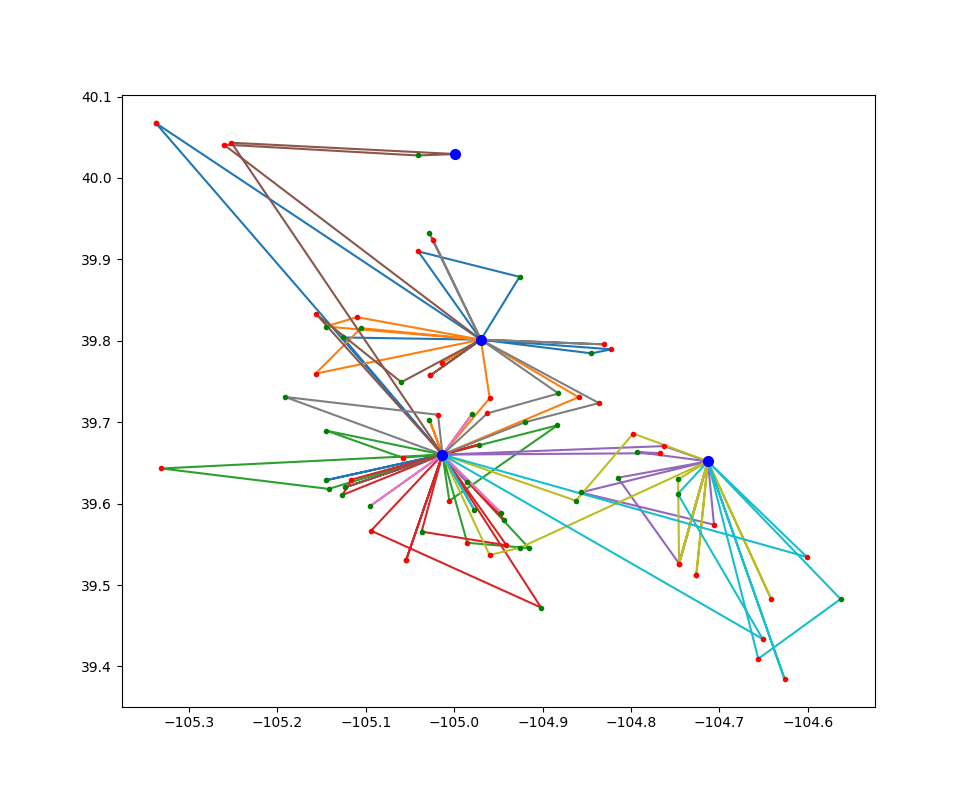
\includegraphics[width=8cm]{sams_route.png}\\
	Route provided by client. Total time spent driving: 1945 minutes.
\end{center} 

\section{Discussion} \label{grp1:discussion}
Here are some comparisons:
  \begin{center}
   \begin{tabular}{llll}
     Name & Minutes & $\%$ TP & $\%$ Sam's\\
     \hline
     Teleportation & 1534 & $0.0$ & $21.1$ \\
     No Can Constraints & 1576 & $2.7$ & $18.9$ \\
     Can Constraints & 1781 & $16.1$ & $8.4$\\
     Sam's & 1945 & $26.8$ & $0.0$\\
   \end{tabular}
   \end{center}
Here, ``Teleportation" refers to the route if drivers could teleport between storage yard
zones, that is, we don't need any transitions (just the triangles by
themselves). The third column is the percent time lost compared to the
teleportation route, and the fourth column is the percent time saved over the
schedule given by the client.

One thing to note about this output is that requiring transitions only added
2.7\% to the time of the solution. To us, that indicates that our pair selection
did quite well, as we could only potentially save that much more.

The program runs very quickly, and it outperforms the client's attempt by
8.4\%. We would have liked to run more data sets to get a more comprehensive report, however, our access to data is limited.

\section{Conclusions/Future Work} \label{grp1:conclusions}
There are two things that would make this program better. One, is better data. If given actual driving times, the output would do a much better job of reflecting real world conditions. As of now, we actually can't even test how well it's doing.

The other thing that would make this better is a better pair choice reflecting
the transitions that will inevitably need to be taken. Right now, pairs are
chosen as if drivers can teleport between storage yards. While a vast majority of a drivers time is \emph{not} taking transitions, it still seems like we are losing a bit here. In order to truely take them into account however, it seems like a much more painful implementation than what is presented. 

In the end, having to take the transitions (as opposed to teleporting between
storage yards) cost the route about 42 minutes, out of 1576, which is around a
$2.7\%$ difference. An improvement could only save us about that much. The obvious next step is to find a bound for the difference between teleportation and our output, however, due to time constraints, we leave it unanswered for now.


\bibliographystyle{plain-annote}
\bibliography{grp1.bib}


%%=======================================
%%  DO NOT EDIT BELOW THIS LINE
%%
%% VVVVVVVVVVVVVVVVVVVVVVVVVVVVVVVVVVVVVV
\ifdefined\CLINICMAIN
\else
\end{document}
\fi
% ^^^^^^^^^^^^^^^^^^^^^^^^^^^^^^^^^^^^^^^^
%  DO NOT EDIT ABOVE THIS LINE
%=========================================

